%
\section{Software specification}
\label{sec:sw-specs}
Next, the \gls{sw} responsible for system operation is specified for all
subsystems --- \texttt{\acrfull{mdo-rc}}, \texttt{\acrfull{mdo-rs}}, and
\texttt{\acrfull{mdo-l}}.
All these subsystems are event-driven (asynchronous), and they can be more easily
specified using state-machine diagrams, previously illustrated in the
\emph{analysis phase} (Section~\ref{sec:softw-arch}). Also in the \emph{analysis
phase}, the use case diagrams helped to identify the main features required for
the system and the respective sequence diagrams helped to clarify the
intervening objects and the interaction among them.

In this section, the analysis phase information is used to derive the static
architecture of the system --- classes diagram --- and to specify algorithms for
its implementation through flowcharts, keeping in mind that the several
subsystems operate multiple tasks concurrently, thus requiring the tasks'
specification and its priorities. The data frame formats are specified for
communication between the different modules. The \acrfull{erd} are depicted to
design the required databases and the \gls{ui} mock-ups are recalled. The test
cases for each subsystem are listed, defining its operation and the expected
result. The \gls{cots} \gls{sw} and the third-party libraries are identified
and a mapping between class topics and the foreseeable implementation is
presented for clarification. Finally, the \gls{sw} tools are listed.

\subsection{Software architecture}
\label{sec:softw-arch-1}
The system's \gls{sw} architecture was devised using \emph{\gls{uml} component
  diagrams} for \texttt{Remote Client} (Fig.~\ref{fig:component-diag-rc}), \texttt{Remote Server} (Fig.~\ref{fig:component-diag-rs}), and
\texttt{Local System} (Fig.~\ref{fig:component-diag-local}). Each component
diagram illustrates all \gls{sw} components for the system in analysis and the
interaction between them, and its
interfaces with external subsystems.

\subsubsection{Remote Client}
\label{sec:remote-client-arch}
Fig.~\ref{fig:component-diag-rc} depicts the \texttt{Remote Client} \gls{sw} architecture, encapsulated in the package
\texttt{MDO-RC: AppManager}, and is comprised of the following artifacts:
\begin{item-c}
\item
  \emph{\texttt{User Interface} package}: contains the \texttt{\gls{ui}} and
  \texttt{\gls{ui} Engine}. It is responsible for providing user feedback and
  capturing \gls{ui} events which drive the \texttt{Remote Client}'s logic.
\item
  \emph{\texttt{Comm Manager} package}: manages incoming and outgoing
  connections to the \texttt{Remote Server} (package \texttt{MDO-RS: App Manager}), periodically checking the
  connection status by pinging the \texttt{Remote Server}. All connections
  consist of \gls{tcp-ip} sockets.
\item
  \emph{\texttt{DB Manager} package}: manages the queries and the associated
  responses by building or parsing them, respectively.
\item 
  \emph{\texttt{Remote Controller} package}: contains the \texttt{Cmd Parser},
  which parses the command responses received from the \texttt{Remote Server}
  when the \texttt{Admin} is performing remote control of the \texttt{Local
    System}.
\item
  \emph{\texttt{RC Rx Parser} component}: high-level parser which filters
  between \texttt{db responses} and \texttt{cmd responses} for appropriate
  dispatching.
\item
  \emph{\texttt{\gls{tcp-ip} Tx} socket}: outgoing connection node, through
  which \texttt{tx frames} are sent to the \texttt{Remote Server}.
\item 
  \emph{\texttt{\gls{tcp-ip} Rx} socket}:  incoming connection node, through
  which \texttt{rx frames} are received from the \texttt{Remote
    Server}.
\end{item-c}

\begin{figure}[htb!]
\centering
    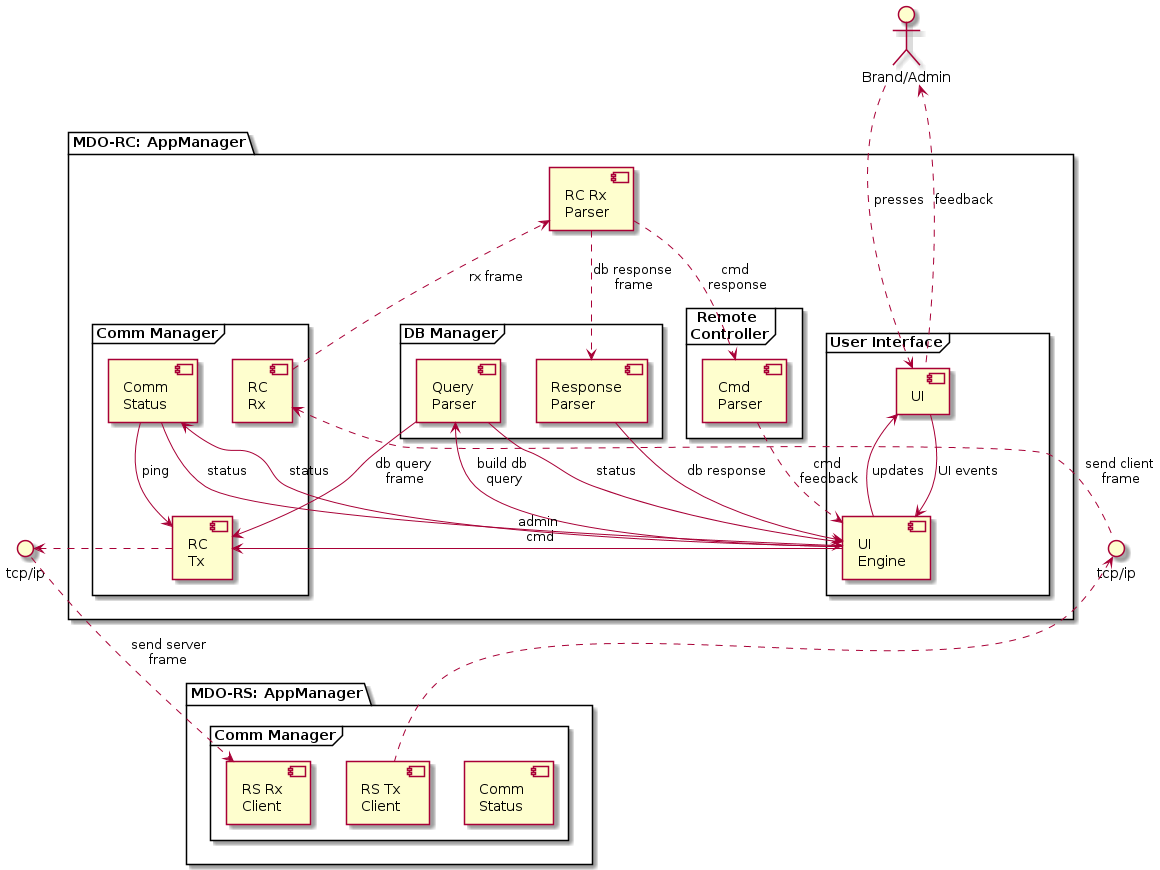
\includegraphics[width=0.9\columnwidth]{./img/component-diag-rc.png}
  \caption{\gls{sw} architecture: component diagram --- \texttt{Remote Client}}%
\label{fig:component-diag-rc}
\end{figure}

\subsubsection{Remote Server}
\label{sec:remote-server-arch}
Fig.~\ref{fig:component-diag-rs} depicts the \texttt{Remote Server} \gls{sw} architecture, encapsulated in the package
\emph{\texttt{MDO-RS: AppManager}}. It interacts with the \texttt{Remote Client}
(package \texttt{MDO-RC: AppManager}), with the \texttt{Local System} (package
\texttt{MDO-L: AppManager}), and with the \texttt{\gls{db} server}
(\texttt{MDO-RS: DB Server}). The database management is done using
client-server architecture, with \texttt{MDO-RS: AppManager} containing the
\gls{db} client and \texttt{MDO-RS: DB Server} the server.
%
\begin{figure}[htb!]
\centering
    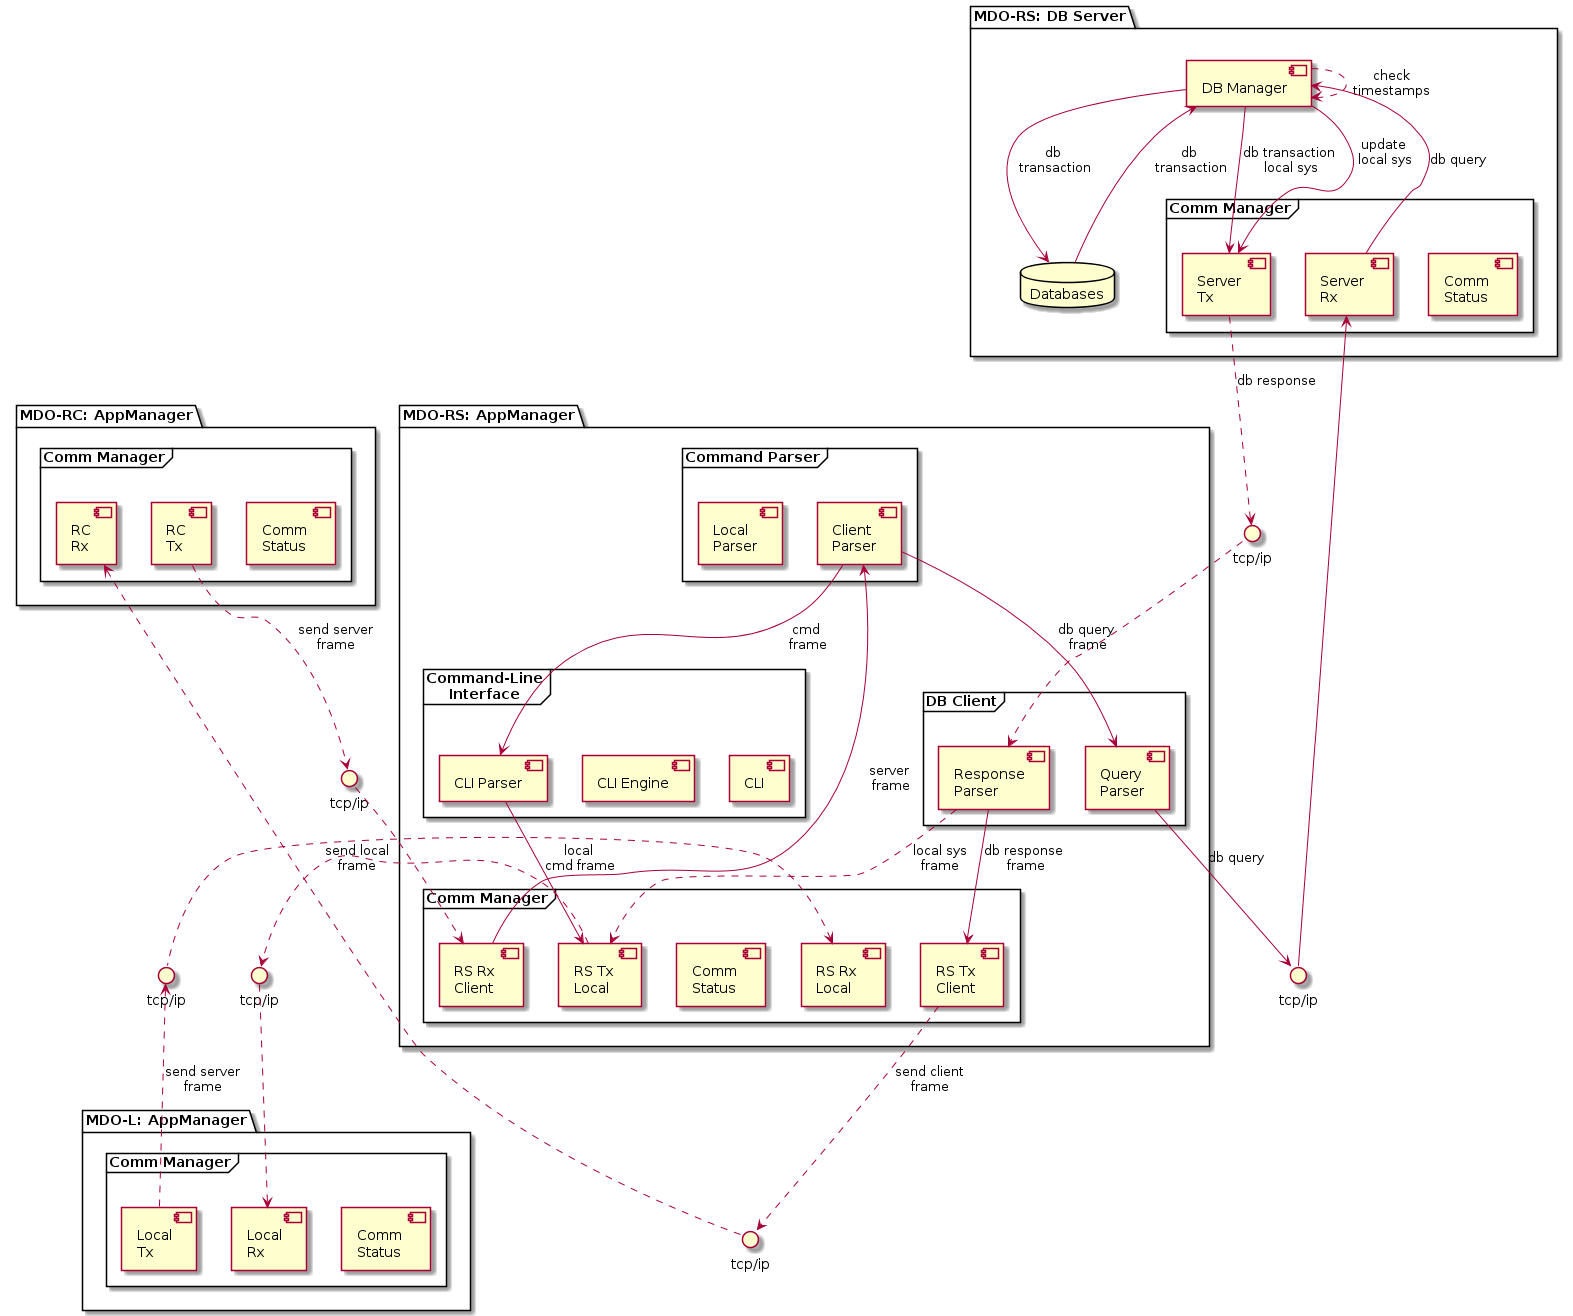
\includegraphics[width=1.0\columnwidth]{./img/component-diag-rs.png}
  \caption{\gls{sw} architecture: component diagram --- \texttt{Remote Server}}%
\label{fig:component-diag-rs}
\end{figure}

The \emph{\texttt{MDO-RS: AppManager}} package is comprised of the following artifacts:
\begin{item-c}
\item
  \emph{\texttt{Command--Line Interface} package}: contains the
  \texttt{\gls{cli}}, the
  \texttt{\gls{cli} Engine}, and the \texttt{\gls{cli} Parser}. It provides the
  server external interface for clients to perform requests,
  capturing the events which drive the \texttt{Remote Server}'s logic.
\item
  \emph{\texttt{Comm Manager} package}: manages incoming and outgoing
  connections to the \texttt{Remote Client} (package \texttt{MDO-RC: App
    Manager}),  and each \texttt{Local System} (package \texttt{MDO-L:
    AppManager}) it needs to interact. It periodically checks all
  connections statuses. All connections
  consist of \gls{tcp-ip} sockets.
\item
  \emph{\texttt{DB Client} package}: manages the queries and the associated
  responses by building or parsing them, respectively. It performs the requests
  for \texttt{\gls{db} server} with the solicited queries.
\item 
  \emph{\texttt{Command Parser} package}: contains the \texttt{Client Parser},
  and the \texttt{Local Parser} to parse and handle frames received from the
  \texttt{Remote Client} or \texttt{Local System}, respectively, forwarding it
  for appropriate dispatching.
\item
  \emph{\gls{tcp-ip} sockets}: incoming/outgoing connection nodes, through which
  incoming or outgoing traffic flows for the \texttt{Remote Client}, the
  \texttt{Local System} and the \texttt{DB Server}.
\end{item-c}

\vspace{1em}
The \emph{\texttt{MDO-RS: DB Server}} package is comprised of the following artifacts:
\begin{item-c}
\item
  \emph{\texttt{Comm Manager} package}: manages incoming and outgoing
  connections to the \texttt{DB Client} (in package \texttt{MDO-RS: App
    Manager}). It periodically checks all
  connections statuses. All connections
  consist of \gls{tcp-ip} sockets.
\item
  \emph{\texttt{DB Manager} package}: handles the received queries, issuing
  transactions for the databases and returns its response. It is also
  responsible for periodically checking timestamps, and when there is a match,
  update the local system with the relevant information.
\item
  \emph{Databases}: contains the actual data stored.
\end{item-c}
%
\subsubsection{Local System}
\label{sec:local-system-arch}
Fig.~\ref{fig:component-diag-local} depicts the \texttt{Local System} \gls{sw} architecture, encapsulated in the package
\emph{\texttt{MDO-L: AppManager}}.
%
\begin{figure}[htb!]
\centering
    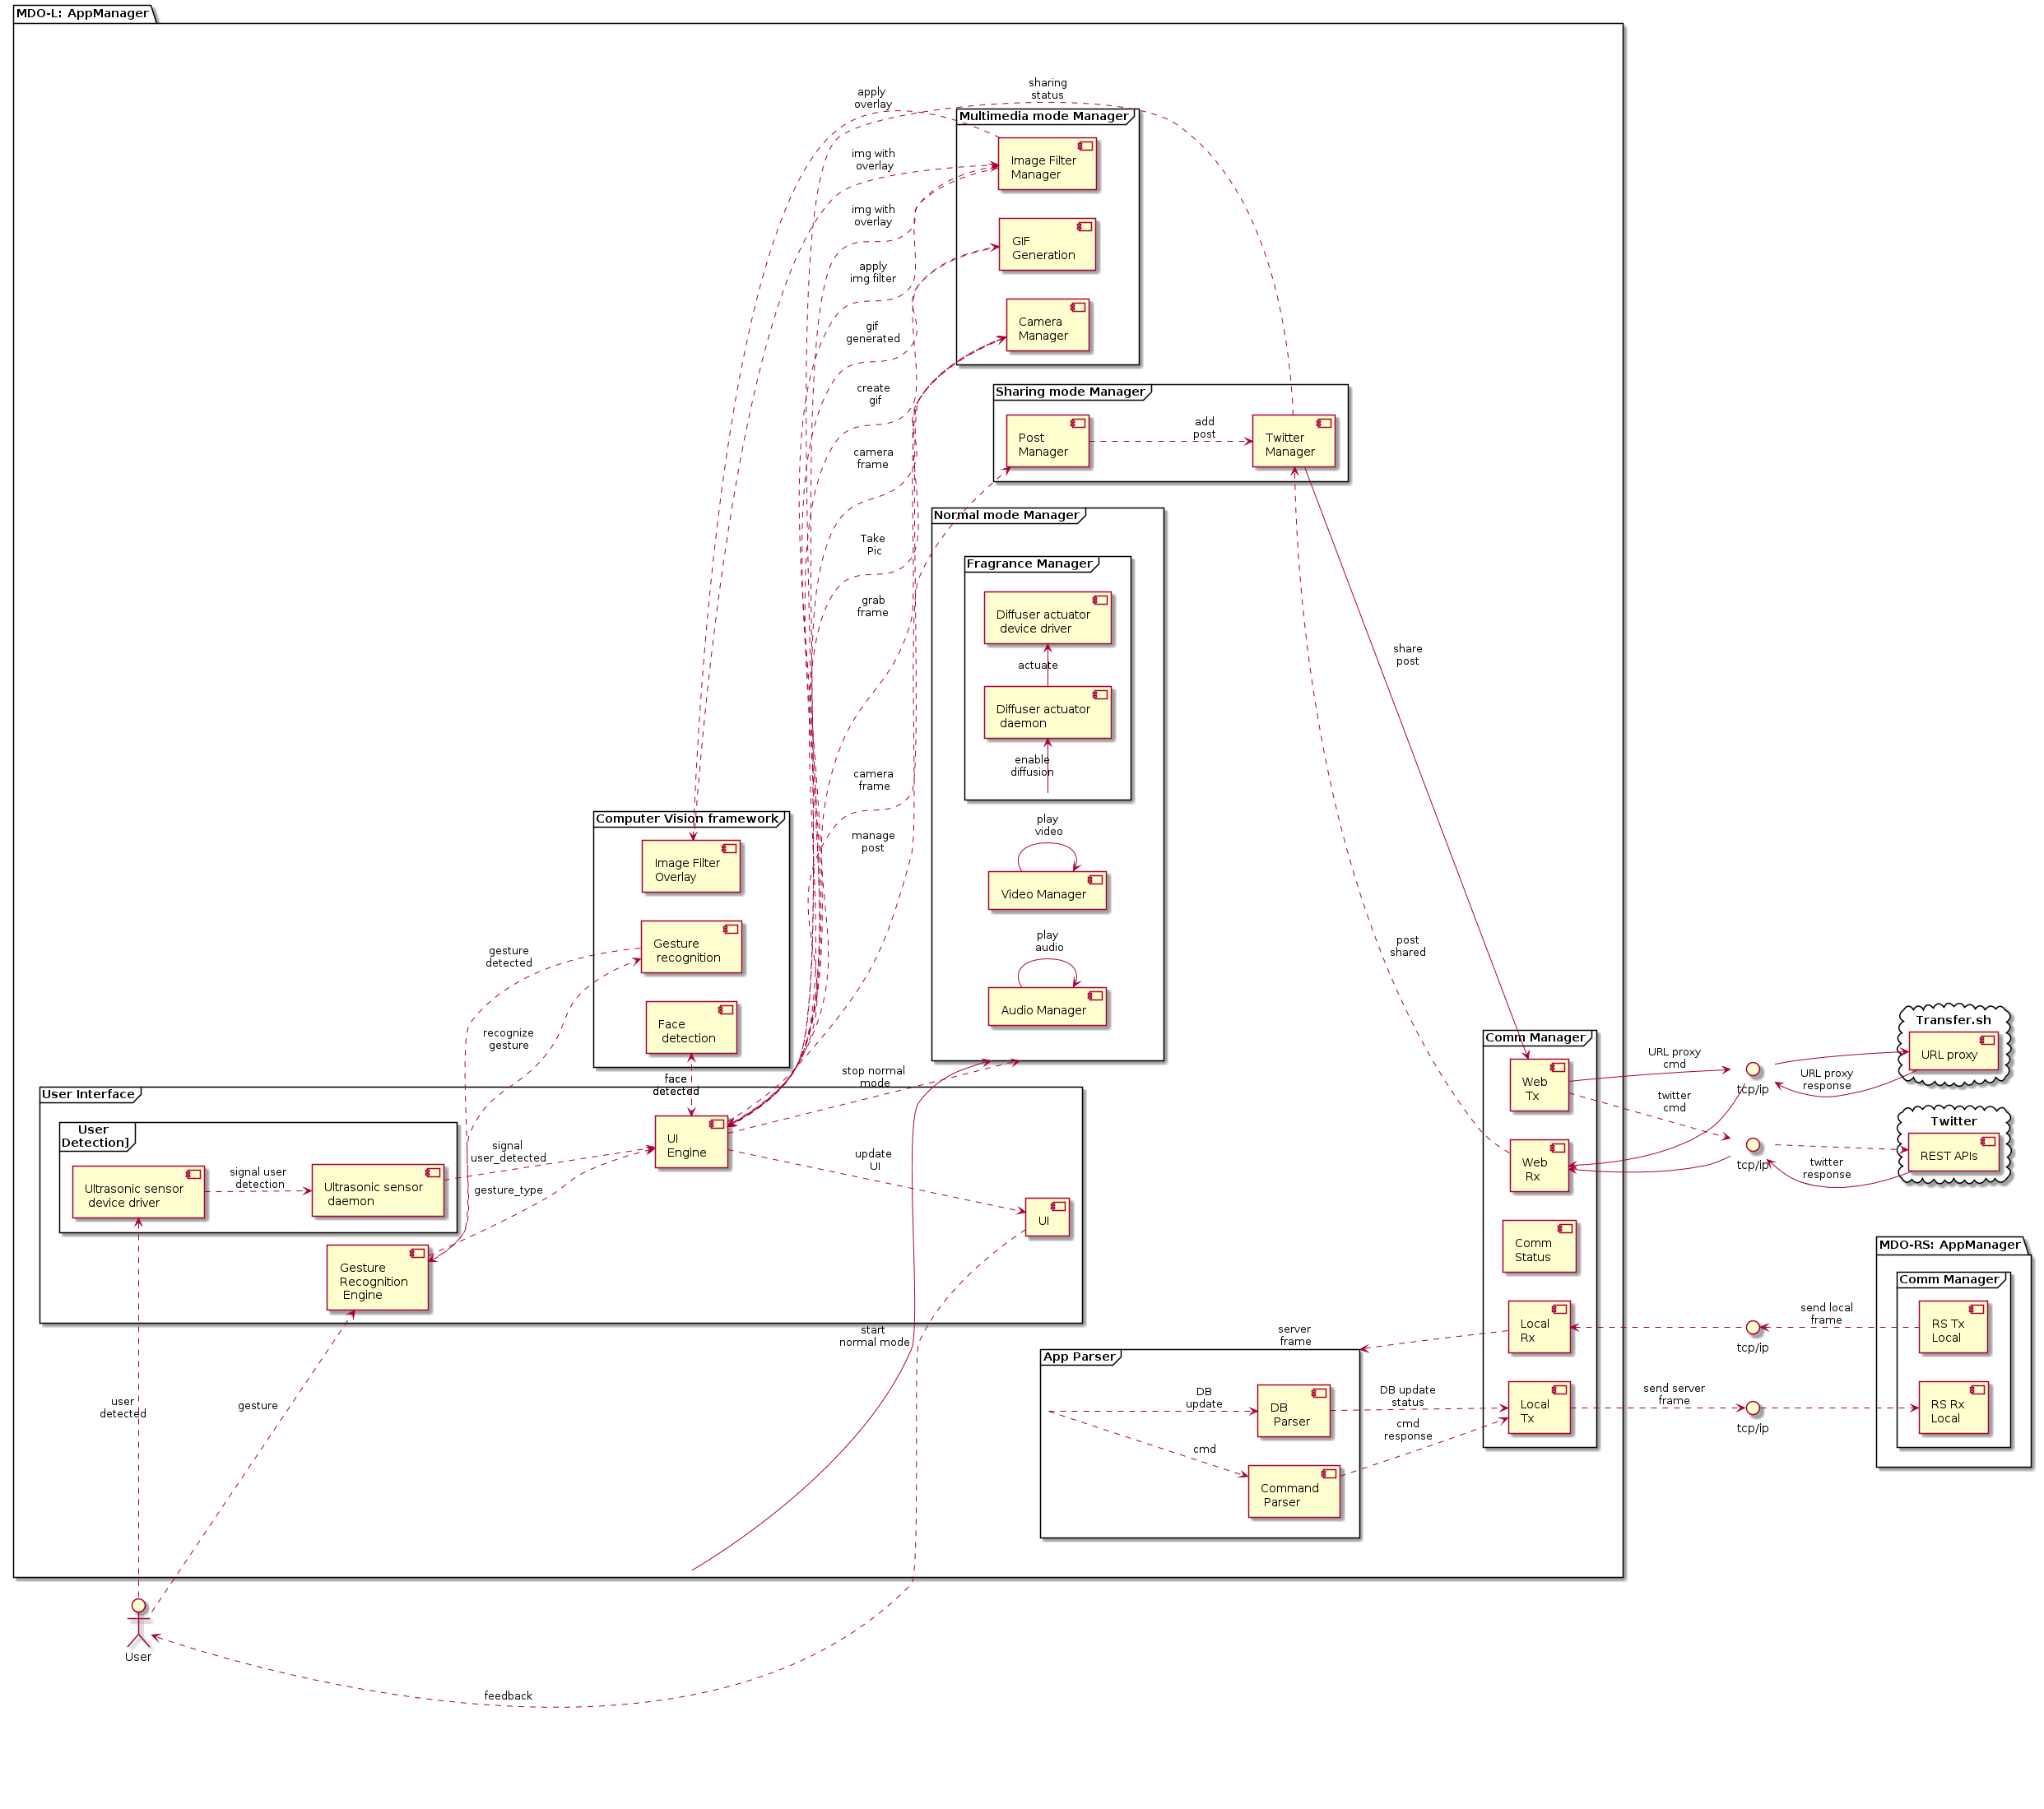
\includegraphics[width=1.03\columnwidth]{./img/component-diag-local.png}
  \caption{\gls{sw} architecture: component diagram --- \texttt{Local system}}%
\label{fig:component-diag-local}
\end{figure}

It interacts with:
\begin{item-c}
\item 
\emph{\texttt{Remote Server}} (package \texttt{MDO-RS: AppManager}): to retrieve updates on its operation or
\texttt{Admin} commands
\item
  \emph{\texttt{Twitter}} (via its \texttt{\gls{rest} \glspl{api}}): to share
  posts on it
\item
  \texttt{transfer.sh} --- an \gls{url} proxy server: to ease file transfer
  between the \texttt{Remote Server} and the \texttt{Local System}.
\end{item-c}

\vspace{1em}
The \emph{\texttt{MDO-RS: AppManager}} package is comprised of the following artifacts:
\begin{item-c}
\item
  \emph{\texttt{User Interface} package}: contains the \texttt{\gls{ui}}, the
  \texttt{\gls{ui} Engine}, the \texttt{Gesture Recognition Engine}, and the
  \texttt{User Detection package}. The \texttt{\gls{ui}} provides user feedback
  and \texttt{UI Engine}
  captures the events that drive the \texttt{Local System}'s logic. When a user
  approaches the \texttt{Local System}, the \texttt{Ultrasonic sensor device
    driver} captures this event and passes it to the user space where the
  \texttt{Ultrasonic sensor daemon} logs it, which, in turn, signals this event
  to the \texttt{UI Engine}. When the \texttt{User} performs gestures, the
  \texttt{Gesture Recognition Engine} requires a service to the \texttt{Gesture
    recognition} component (\texttt{Computer Vision Framework}) to recognize the
  gesture. Also, when the \texttt{User} is detected, the \texttt{UI Engine}
  requests the \texttt{Normal mode manager} to stop running, and requests
  \texttt{Face detection} to track people's faces in the camera.
\item
  \emph{\texttt{Comm Manager} package}: manages incoming and outgoing
  connections to the \texttt{Remote Server} (package \texttt{MDO-RS: App
    Manager}),  and the internet for each web service it needs to interact
  (\texttt{Twitter} and \texttt{transfer.sh}).
  It periodically checks all connections statuses. All connections
  consist of \gls{tcp-ip} sockets.
\item
  \emph{\texttt{Computer Vision framework} package}: manages the computer vision
  related tasks, namely, gesture recognition, face detection, and image filter
  overlay.
\item 
  \emph{\texttt{Multimedia Mode Manager} package}: manages the multimedia mode
  related tasks, namely, image filtering, \gls{gif} generation, and camera
  management.
\item 
  \emph{\texttt{Sharing Mode Manager} package}: manages the sharing mode
  related tasks, namely, post management, and social media management, in this
  case, \texttt{Twitter}.
\item 
  \emph{\texttt{Normal Mode Manager} package}: manages the normal mode
  related tasks, namely, fragrance diffusion, video and audio outputs. The
  fragrance diffusion is requested to the device driver using a daemon to bridge
  user-space and kernel-space.
\item 
  \emph{\texttt{App Parser} package}: manages the parsing for database queries
  and requested commands.
\item
  \emph{\gls{tcp-ip} sockets}: incoming/outgoing connection nodes, through which
  incoming or outgoing traffic flows for the \texttt{Remote Server}, and the web
  services for \texttt{Twitter} and the \texttt{\gls{url} proxy server}.
\end{item-c}
%
%

%
\subsection{Deployment specification}
\label{sec:deployment-spec}
The deployment specification maps the software artifacts derived in the
component diagrams to the respective computational node where it will be
executed. This step pertains to the implementation phase; nonetheless, it is
illustrated here as it clarifies the \gls{sw} architecture, as well as it guides
some design decisions.

Fig.~\ref{fig:deploy-diag} depicts the deployment diagram for the \gls{mdo}
system. In blue are represented the computational nodes of interest, namely:
\begin{item-c}
\item
  \emph{\texttt{Linux PC}}:
  it is the host device, where are executed the packages
  (in grey) \texttt{MDO-RC: AppManager}, the \texttt{MDO-RS: AppManager}, and
  the \texttt{MDO-RS: DB Server}. All connections between packages in the
  \texttt{Linux PC} and \texttt{Raspberry Pi} are \gls{tcp-ip} sockets in
  a client-server architecture. The design and subsequent implementation of
  these packages are not limited by the embedded device constraints, thus, the
  focus is on functionality and ease of implementation. It is important to note
  the design is decoupled, i.e., the \texttt{Remote Client} and \texttt{Remote
    Server} can be executed in different computational nodes, where, the former
  runs on a desktop computer and the latter on a cloud-based service or
  mainframe, thanks to the client-server architecture based on \gls{tcp-ip}
  sockets. Thus, for practicality reasons, both subsystems are implemented on
  the same \texttt{Linux PC}, but it should be straightforward to migrate them
  to different and distinct platforms.
\item
  \emph{\texttt{Raspberry Pi}}:
  it is the embedded device, where is executed the package \texttt{MDO-L:
    AppManager}. It interacts with \texttt{Remote Server} and \texttt{Web
    services} --- \texttt{Twitter} and \texttt{Transfer.sh} --- using
  \gls{tcp-ip} sockets in a client-server architecture. The design and subsequent
  implementation of this package is limited by the embedded device constraints,
  thus, the focus in on functionality and performance.
\item
  \emph{\texttt{Web}}:
  it represents the remote computational nodes where the \texttt{Web services}
  --- \texttt{Twitter} and \texttt{Transfer.sh} are executed. The \texttt{Local
    System} interacts with these services using \gls{tcp-ip} sockets in a
  client-server architecture through the exposed \glspl{api}.
\end{item-c}
%
%
\begin{figure}[htb!]
\centering
    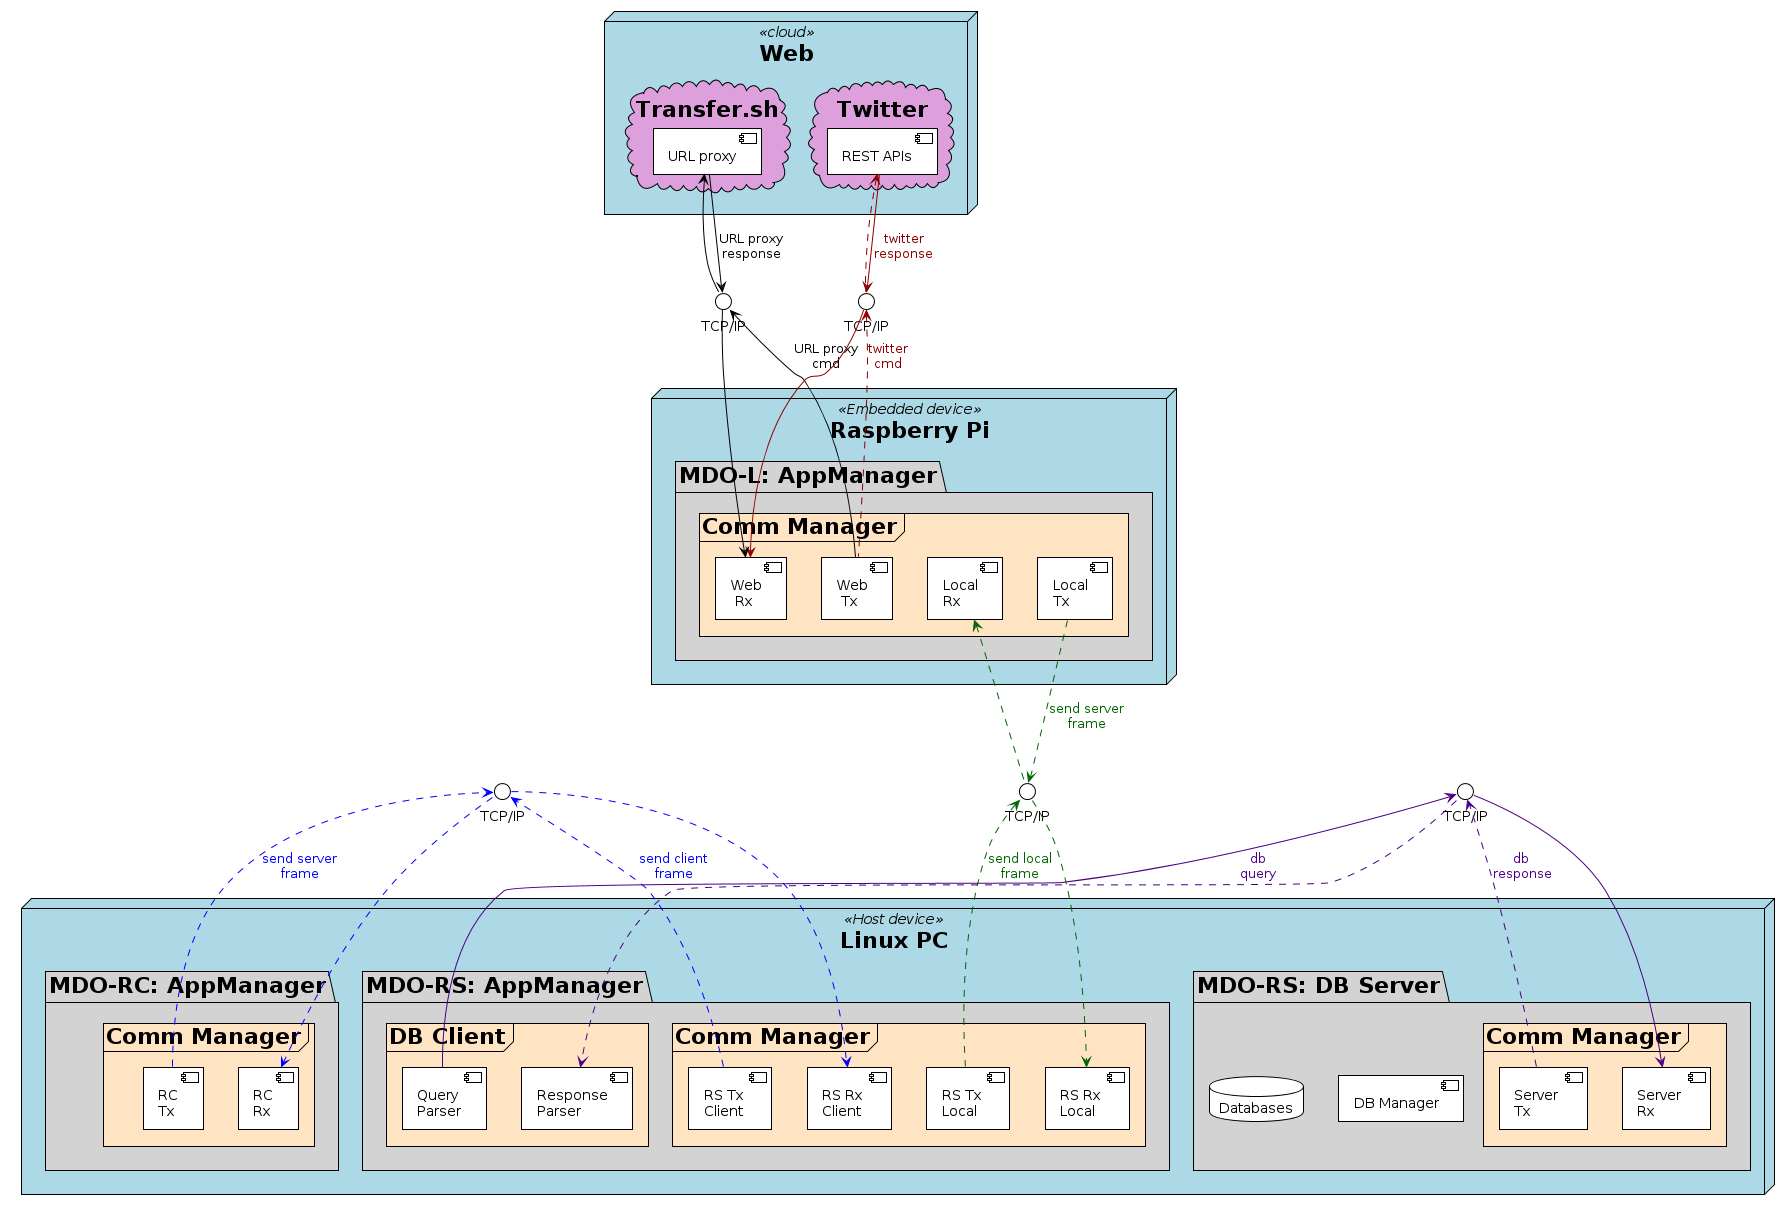
\includegraphics[width=1.0\columnwidth]{./img/deploy-diag.png}
  \caption{Deployment diagram}%
\label{fig:deploy-diag}
\end{figure}

\subsection{Database design}
\label{sec:database-design}
As aforementioned in Section~\ref{sec:datab-design-overv}, the conceptual design
of a database consists of a high-level description of the data to be stored in
the database and its constraints, which is usually carried out using the
\gls{er} model. Thus, in Section~\ref{sec:entity-relat-model} the key concepts
of the \gls{er} model are presented, which can be reviewed to assist the
comprehension of the subsequent database design produced.

Fig.~\ref{fig:erd} depicts the \gls{erd} for the conceptual design of the
\gls{mdo} system's database,
with the primary keys shown in red and the foreign keys in blue,
comprising the relevant entities and its relationships, namely:
\begin{item-c}
\item
  \emph{\texttt{User}}:
  models an User in the application (\texttt{Brand} or \texttt{Admin}). It has a
  \texttt{role}, a \texttt{name}, an \texttt{email}, and a \texttt{pass} (which
  is encrypted before being stored). An \texttt{User} manages \texttt{0} or many
  \texttt{UserStations} and owns \texttt{0} or many \texttt{Ad}s.
\item
  \emph{\texttt{UserStations}}: it unfolds the relationship many-to-many between
  an \texttt{User} and a \texttt{Station}. An \texttt{User} manages \texttt{0}
  or many \texttt{UserStations}, and a \texttt{UserStations} contains one or
  many \texttt{Station}s. It imports the \texttt{User.id} as a foreign key to
  enable referencing an \texttt{User}.
\item
  \emph{\texttt{Station}}: it models a physical \gls{mdo} station. It contains
  an \texttt{id}, a \texttt{name}, a \texttt{location} and an \texttt{IP}
  address. It imports the \texttt{UserStations.id} as a foreign key to
  enable referencing an \texttt{UserStations}.
\item
  \emph{\texttt{TimeTable}}: it models a weekly timetable that every
  \texttt{Station} contains. It contains one or many \texttt{TimeSlot}s.
  It imports the \texttt{Station.id} as a foreign key to
  enable referencing a \texttt{Station}.
\item
  \emph{\texttt{TimeSlot}}: it models a slot of time available for ads
  reproduction. It contains the \texttt{duration} (in minutes), the
  \texttt{cost}, and a flag signaling if it is \texttt{rented} or not. It
  imports the \texttt{TimeTable.id} as a foreign key to enable referencing a
  \texttt{TimeTable}.
\item
  \emph{\texttt{Ad}}: it models an advertisement.
  It imports the \texttt{User.id} as a foreign key to reference an
  \texttt{User}, a \texttt{Fragrance.id} to reference the associated
  \texttt{Fragrance}, and a \texttt{TimeSlot.id} to reference a
  \texttt{TimeSlot}. The \texttt{Fragrance} is optional, but, as the foreign key
  must not contain a null value, a default value of \texttt{0} is used to signal
  that no fragrance is used.
\item
  \emph{\texttt{MediaFile}}: it models a media file that must be attached to the
  \texttt{Ad}. It contains an \texttt{id}, file specifications (\texttt{filename}, \texttt{filesize}, and \texttt{filetype}), \texttt{mdata}
  for storing the file and an optional \texttt{description}. It
  imports the \texttt{Ad.id} as a foreign key to enable referencing an
  \texttt{Ad}.
\item
  \emph{\texttt{Fragrance}}: it models a \texttt{Fragrance}. It is added to the
  database by the \texttt{Admin} and it can be selected by the \texttt{Brand}
  from the \texttt{FragranceList} available for each \texttt{Station}.
  It contains an
  \texttt{id}, a \texttt{name}, an \texttt{intensity} to define the actuation
  time, a maximum capacity (\texttt{vol\_ml\_max}) and a current capacity
  (\texttt{vol\_ml\_level}), and an optional \texttt{description}. It
  imports the \texttt{FragranceList.id} as a foreign key to reference the
  \texttt{FragranceList} available for each \texttt{Station}.
\item
  \emph{\texttt{FragranceList}}: it represents the list of fragrances available
  for each \texttt{Station}.
  It imports the \texttt{Station.id} as a foreign key to reference its
  associated \texttt{Station}.
\end{item-c}

%
\begin{figure}[htb!]
\centering
    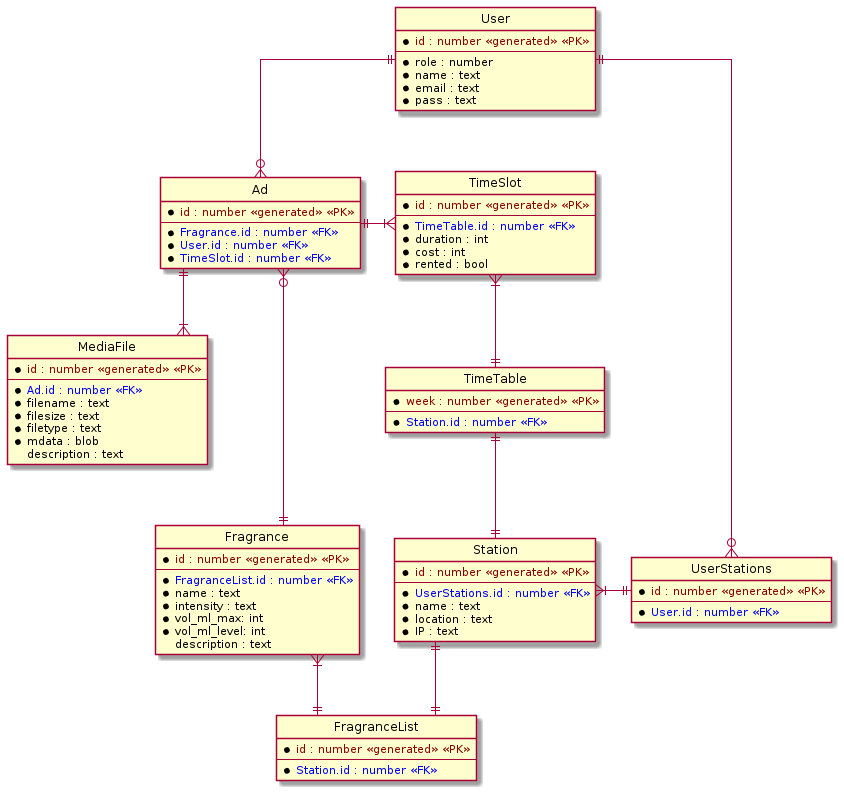
\includegraphics[width=1.0\columnwidth]{./img/erd.png}
  \caption{\gls{mdo} Entity-Relationship Diagram: conceptual design}%
\label{fig:erd}
\end{figure}

\subsection{Data formats}
\label{sec:data-formats}
After devising the \gls{sw} architecture the data flow across the several
subsystems became clearer, with data frames being conveyed through \gls{tcp-ip}
sockets. Thus, it is important to define the data formats for internal
representation and communication between the subsystems, as illustrated in
Fig.~\ref{fig:data-formats}. In gray are depicted the several subsystems, in
white the data frames and in blue the legend.

The several subsystems will communicate using a basic data frame ---
\texttt{rxFrame} --- which contains a \texttt{header}, the data length, the
actual data, and an \texttt{ACK} (acknowledge) signal. The \texttt{header} defines the frame type which can be \texttt{DB}
(database queries), \texttt{CMD} (commands sent to be executed), and \texttt{AD}
(ads to be reproduced --- only for \texttt{Local System}). It is important to
note: the usefulness of \texttt{data}'s datatype being \texttt{void *}, as it is
generic, and thus enables the encapsulation of other data frames --- e.g., the
\texttt{AdFrame} is encapsulated within a \texttt{rxFrame}; the \texttt{ACK}
signal is a valid terminator for all data frames --- helping to identify bigger
data frames than the maximum ones, and to prevent ill-intentioned data frames
usage to corrupt the system --- of type \texttt{int} to prevent collisions with
normal messages sent.

The \texttt{Remote Server} contains an additional data frame ---
\texttt{serverFrame} --- which encapsulates a received \texttt{rxFrame} and
pairs it with the sender socket descriptor information to enable appropriate
message routing.

The \texttt{AdFrame} contains the information about the advertisement to be
reproduced, namely its type, intensity, start time, duration, media length, and media \glspl{url}. The
first identifies the fragrance within the \texttt{Local System}, the second is
used to calculate the fragrance diffusion timing, the start time is the elapsed
time from the start of the day, the duration is the reproduction time of the ad
(in minutes), and the \texttt{mediaURLs} contain the \glspl{url} from where the
media files can be downloaded and stored in the \texttt{Local System}.
%
\begin{figure}[htb!]
\centering
    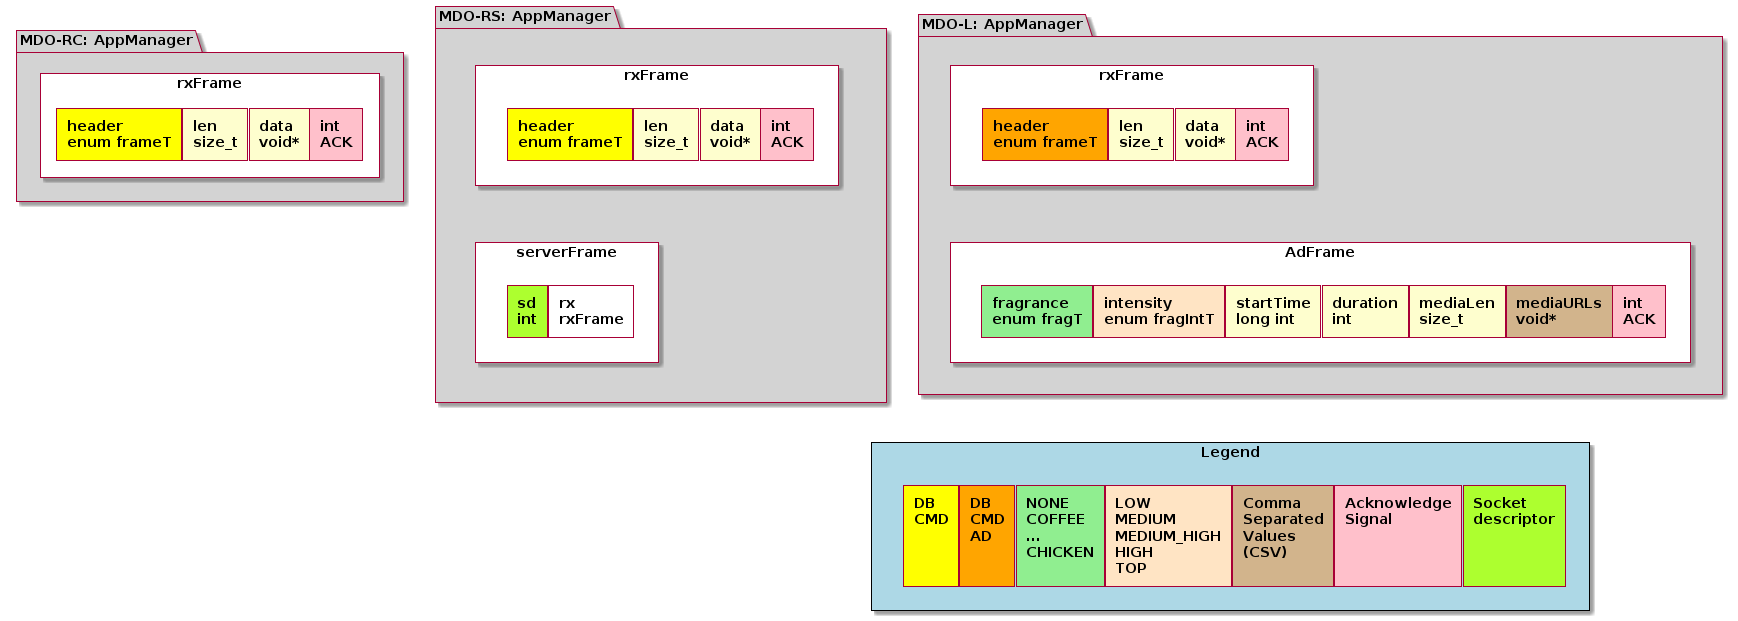
\includegraphics[width=1.0\columnwidth]{./img/data-formats.png}
  \caption{Data formats}%
\label{fig:data-formats}
\end{figure}
%

\subsection{Static architecture --- Class diagrams}
\label{sec:stat-arch-class}
In this section the static architecture is derived from the \gls{sw}
architecture, i.e., the class diagrams are outlined, using the component
diagrams as a starting point, for each subsystem.

\subsubsection{Remote Client}
\label{sec:remote-client-class}
%
Fig.~\ref{fig:class-diag-rc} depicts the class diagram for the \texttt{Remote Client} subsystem.
The \texttt{UIApp} and \texttt{UIWindow} handle all the events made by the user with the \gls{ui}.
The \texttt{CommManager} handles the communication between this system and the \texttt{Remote Server}, which has an enumerator to classify the connection status (\texttt{ConnStatus}) and also the class \texttt{DBManager} handles all the databases through its functions and enumerators \texttt{DB\_OPER} and \texttt{DB\_OBJ}.
Then, there's the normal classes that are mandatory to have: \texttt{User} and \texttt{Admin} that have a relation (because an Admin is a User), \texttt{Station} with its \texttt{TimeTable}, \texttt{Date} and also \texttt{Ad} to handle the ads.

There are some functions that are important to be referenced, such as \texttt{serialize()} - this function serializes all the members of the class in order to be more easier to build queries to the databases, that's why there is a function with that name in almost all classes.
Also, the function \texttt{buildQuery} is important because it builds the queries to send to the databases having in mind the type of query and the table that it wants to access. In this way, it is more easier to handle all the application, with no need to save too much data unnecessarily.  
%
\begin{figure}[htb!]
\centering
    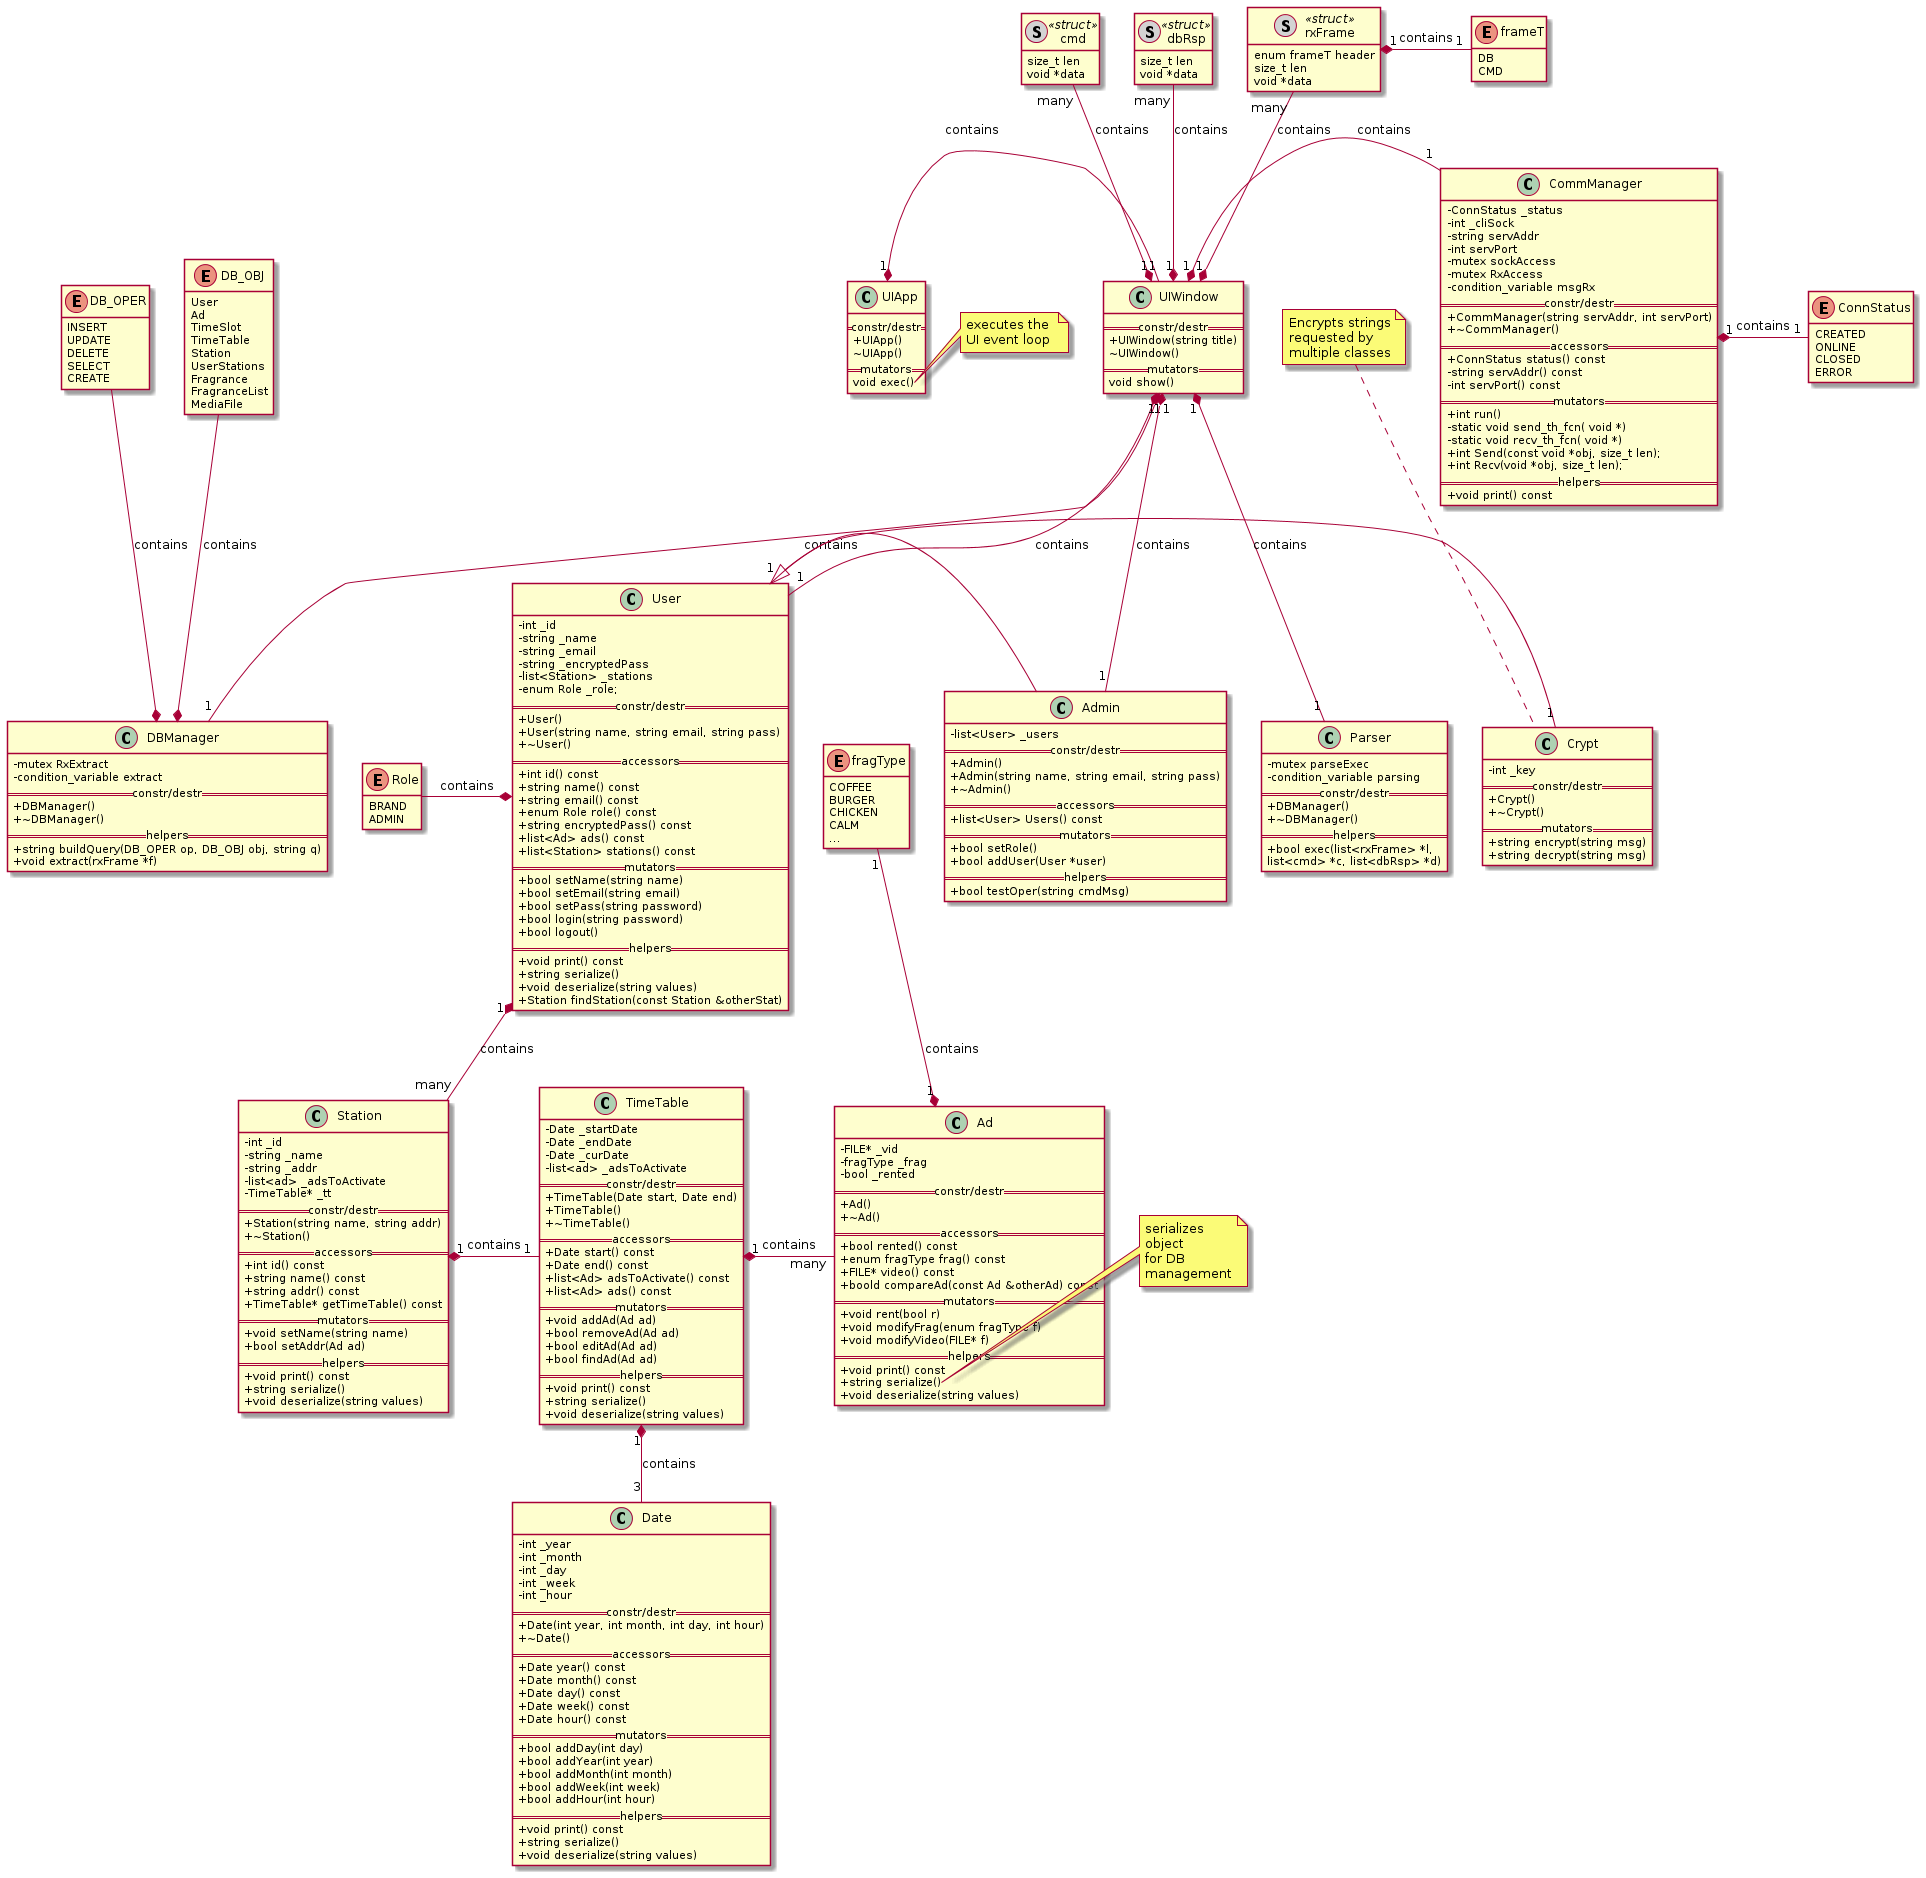
\includegraphics[width=1.0\columnwidth]{./img/class-diag-rc-hugo.png}
  \caption{Class diagram: \texttt{Remote Client}}%
\label{fig:class-diag-rc}
\end{figure}

\subsubsection{Remote Server}
\label{sec:remote-server-class}
%
Fig.~\ref{fig:class-diag-rs} depicts the class diagram for the \texttt{Remote Server} subsystem.
The \texttt{CLI} is the Command Line Interface and handles almost everything in this subsystem. It has several members, the more important ones are the send and receive vectors that have the type of data \texttt{serverFrame} containing the rxFrame and the socket to which the server is connected, this facilitates the work when sending and receiving because there is already the knowledge of the socket to or from the message is being received or sent. Allied to this, there's all the conditional variables and mutexes that maintain the stability of all variables and avoid collisions between classes, communications and so on.

The \texttt{CommManager} handles all the communication and has the most important functions: the \texttt{send} thread, the \texttt{receive} thread and the \texttt{connect} thread.

The \texttt{Parser} class has the finality to parse and execute all the commands that are received either to handle the database or to communicate to the remote client or the local system.

The  \texttt{DBClient} is used to handle all the mechanisms of all the databases, making queries, receiving responses and so on. Finally, the \texttt{Crypt} class is to encrypt something that can be necessary, such as files, passwords or some commands. 
%
\begin{figure}[htb!]
\centering
    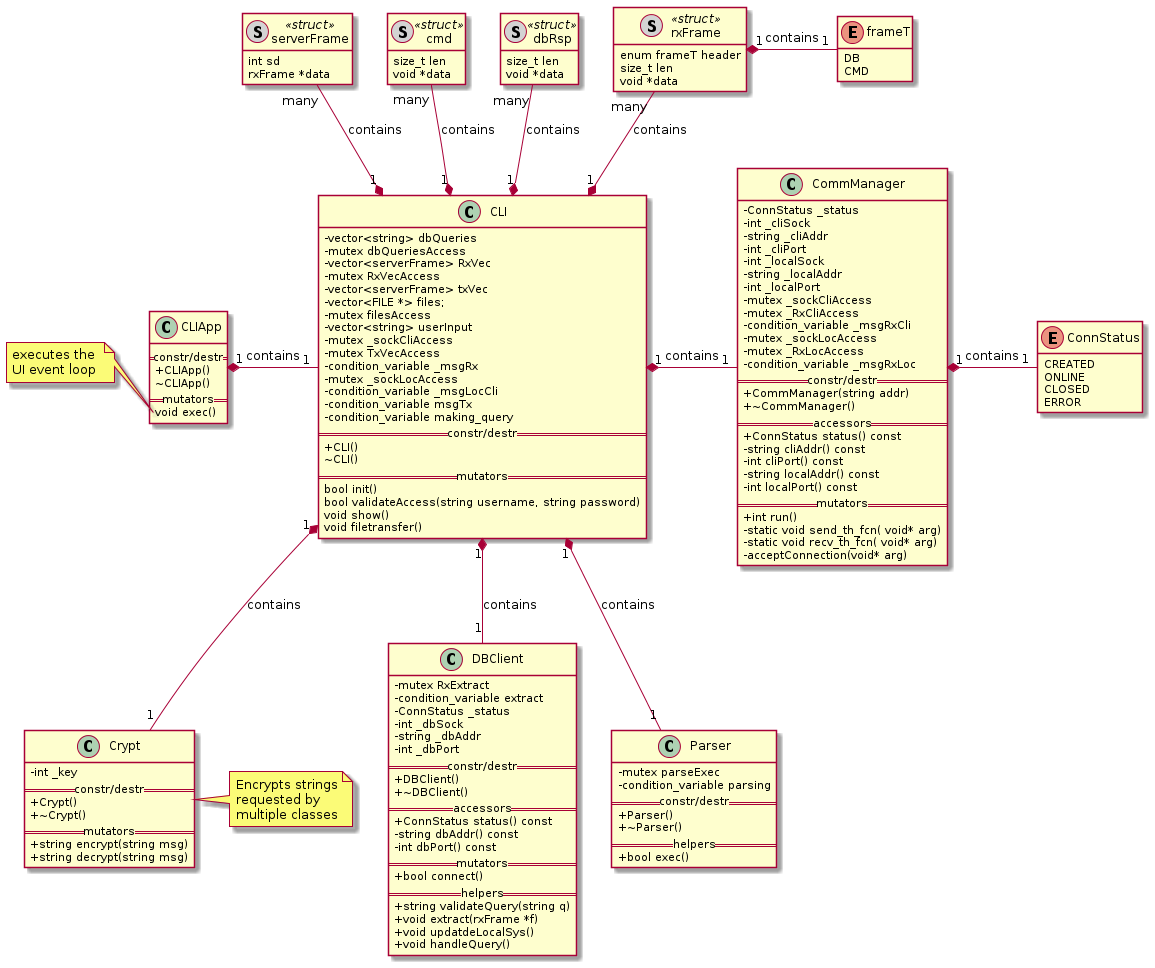
\includegraphics[width=1.0\columnwidth]{./img/class-diag-rs-hugo.png}
  \caption{Class diagram: \texttt{Remote Server}}%
\label{fig:class-diag-rs}
\end{figure}

\subsubsection{Local System}
\label{sec:local-system-class}
%
Fig.~\ref{fig:class-diag-local-1} and Fig.~\ref{fig:class-diag-local-2} depicts the class diagram for the
\texttt{Local System}.

In Fig.~\ref{fig:class-diag-local-1} is illustrated a partial view of the class
diagram of the \texttt{Local System}, containing the \texttt{UIApp} which
executes the \texttt{UI} event loop. As the majority of the events are triggered
by the \texttt{User} it is reasonable to compose the \texttt{UI} object of all
the other ones, and the relevant data structures.

The \texttt{CommManager} handles all communications to the
\texttt{RemoteServer}, the \texttt{UserDetectionEngine} handles the user
detection and the \texttt{GestureRecognitionEngine} handles the recognition of
user gestures.
%
A \texttt{Parser} abstract class is derived to obtain specialized parsers for
\gls{db}, commands and Twitter. \texttt{Twitter} is derived from
\texttt{SocialMedia} abstract class to handle \texttt{Post} objects and share
them on \texttt{Twitter}.
%
\begin{figure}[htb!]
\centering
    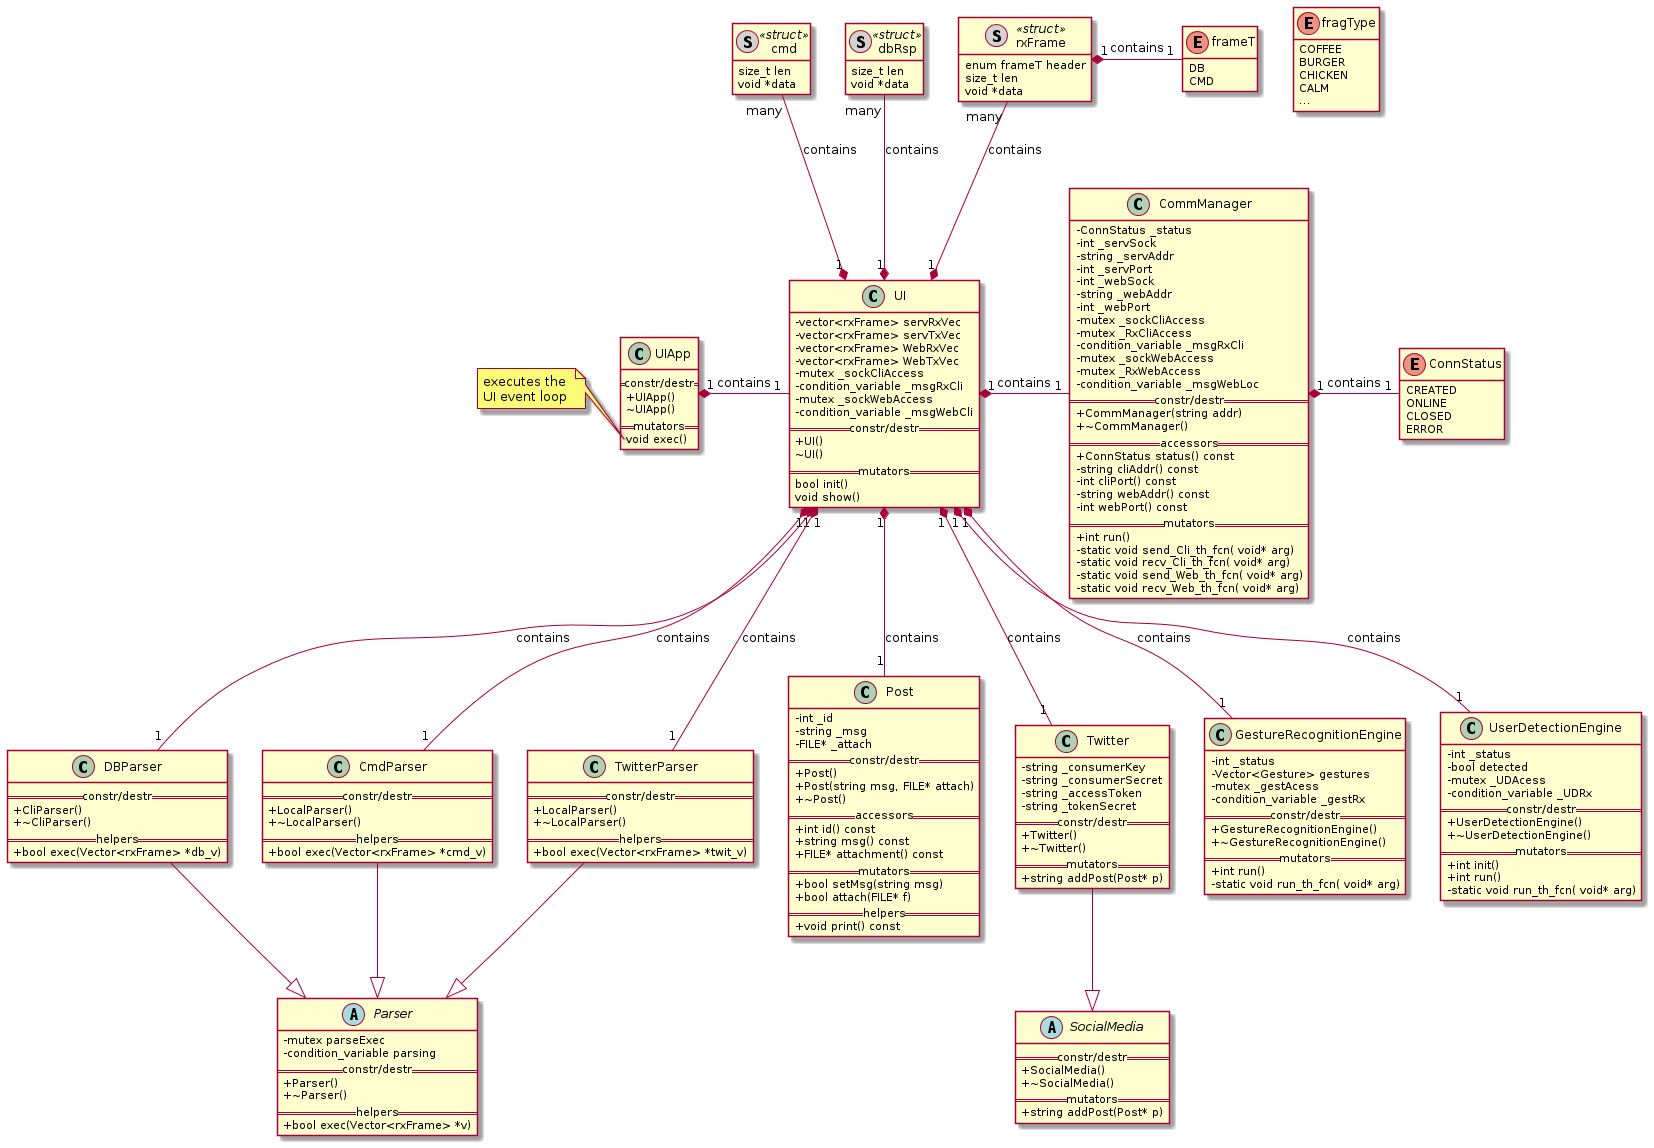
\includegraphics[width=1.0\columnwidth]{./img/class-diag-local-1.png}
  \caption{Class diagram: \texttt{Local System} --- part 1/2}%
\label{fig:class-diag-local-1}
\end{figure}

In Fig.~\ref{fig:class-diag-local-2} is illustrated the second part of the class diagram of the \texttt{Local System}.

As it can be seen, there are some classes that handle some features of the station, such as \texttt{GIFGenerator}, \texttt{VideoManager}, \texttt{AudioManager}, \texttt{ImageFilterEngine}, \texttt{CameraEngine} and \texttt{FragranceManager}. All these classes handles all modes of the local system and, obviously they all interact with the \texttt{UI}.

There is also the class \texttt{Ad} that handles the ads and has the structure
\texttt{adFrame} containing some information that are relevant to download the
associated media
files and play the ad on the station.

There are several threads in various classes that will be explained next in section \ref{sec:thre-spec}.
%
\begin{figure}[htb!]
\centering
    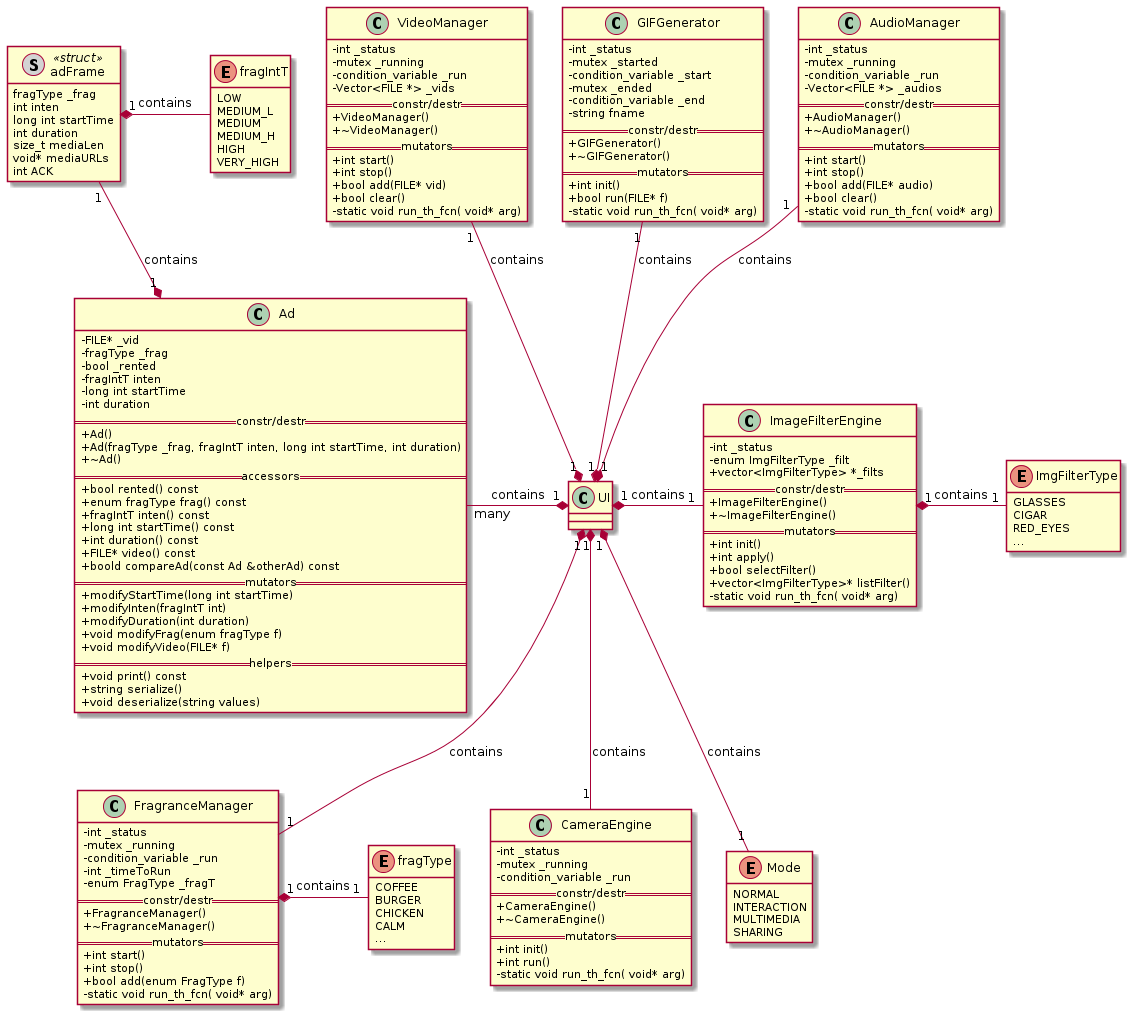
\includegraphics[width=1.0\columnwidth]{./img/class-diag-local-2.png}
  \caption{Class diagram: \texttt{Local System} --- part 2/2}%
\label{fig:class-diag-local-2}
\end{figure}

\subsection{Threads specification}
\label{sec:thre-spec}
In this section the threads specification are performed for the several
subsystems, assigning them the respective priority. A color scheme is used to
define thread priority, with red being the highest and green the
lowest. Additionally, the threads are ranked from highest (at the top) to lowest
(at the bottom) in each frame.

\subsubsection{Remote Server}
\label{sec:remote-server-threads}

Fig.~\ref{fig:thread-spec-rs} illustrates the thread specification and the associated priorities for the \texttt{Remote Server}. 
There are four logical groups:
\begin{enum-c}
\item\emph{\texttt{CLI}}: the command line interface has a thread to transfer files because it can be necessary to transfer them to both subsystems.
This thread has low priority because it is not a critical feature that need to happen as soon as possible and, depending on the file, it can take a while until its transfer, so, it can have a lower priority and take its time to transfer.
\item\emph{\texttt{Parser}}: the parser has one thread that is its execution. This thread has high priority because it is mandatory to parse and execute the commands that are received, as soon as they are received.
\item\emph{\texttt{Comm}}: the communication manager has three threads that are important: the \texttt{receive}, the \texttt{send}, and the \texttt{accept connection}. The one with most priority is the \texttt{receive} thread, because it is necessary to receive the messages to then parse and execute them. Then, the other two threads have medium priority because receiving and parsing messages is more important than this.
\item\emph{\texttt{DB}}: the database management has three threads that have high priority, that's because it is important to always have the databases updated. These three threads make queries to the databases, but they are controlled one by another in order to avoid the risk to make queries at the same time or some queries to be lost. There's another thread that handles the commands sent to the server or between the two subsystems
\end{enum-c}
%
\begin{figure}[htb!]
\centering
    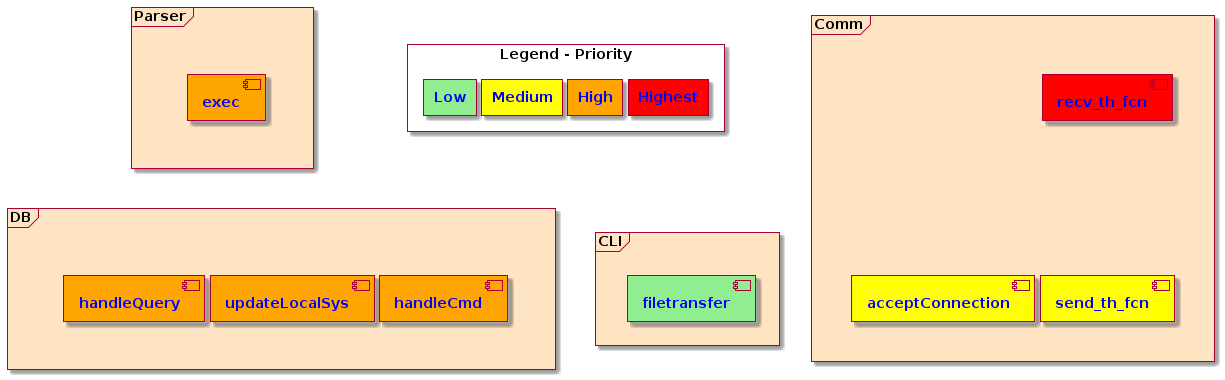
\includegraphics[width=0.8\columnwidth]{./img/thread-spec-rs.png}
  \caption{Thread specification: \texttt{Remote Server}}%
\label{fig:thread-spec-rs}
\end{figure}
%

\subsubsection{Local System}
\label{sec:local-system-2}
%
Fig.~\ref{fig:thread-spec-local} illustrates the thread specification and the
associated priorities for the \texttt{Local System}. There are five logical
groups:
\begin{enum-c}
\item
  \emph{\texttt{User Interface}}: the \texttt{UserDetection} detects when a user
  is in range and is the top priority
  thread, as it will determine the device's mode, stopping \emph{normal mode}
  and going into \emph{interaction mode}.

  The \texttt{FrameGrabber} and \texttt{UI} threads are \emph{high
    priority}. The first grabs frames from the camera and stores it in a frame
  buffer which is available to the \texttt{UI}, \texttt{ImgFilterOverlay}, and
  \texttt{GestureRecognition} threads. The second is
  responsible for providing user feedback on the \gls{lcd} display.

  The \texttt{ImgFilterOverlay}, and the \texttt{GestureRecognition}, and the
  threads are medium priority. The first is responsible
  for detecting faces on the camera frame buffer and applying the selected image
  filter overlay, and the second for recognizing \texttt{User} gestures.

  It should be noted that only the \texttt{UserDetection} and \texttt{UI}
  threads should be permanently running, while the others are only running while
  an \texttt{User} is detected.
\item
  \emph{\texttt{Comm}}: these threads are responsible for communications
  handling.
  \texttt{LocalRx} is the top priority thread, as it needs to check if an
  relevant command or database update has arrived. It stores the incoming data
  frames into a \gls{fifo} buffer.

  The \texttt{LocalTx} is a high priority threads, responsible for
  transmitting outgoing data frames to the \texttt{RemoteServer}.

  The \texttt{TwitterShare} and \texttt{FileTransfer} are low priority tasks, as
  they don't impact the user experience or device operation significantly. The
  first is responsible for sharing posts on Twitter. The second handles file
  transferring between \texttt{RemoteServer} and the \texttt{LocalSystem}.
\item
  \emph{\texttt{App}}: these threads handle app specific tasks.
  The \texttt{AppParser} is a high priority thread, consuming incoming data
  frames and dispatches it for additional processing of commands ---
  \texttt{CmdHandler} --- or of \texttt{Ad}s requiring file transfer ---
  \texttt{FileTransfer}.

  The \texttt{CmdHandler} is a medium priority task responsible for responding
  to commands sent to the \texttt{Local System}.
\item
  \emph{\texttt{Normal mode}}: these threads are only running when normal mode
  is on.
  \texttt{AudioMan} and \texttt{VidMan} are high priority tasks, and they are
  responsible for Ad's audio and video management, respectively.

  \texttt{FragMan} is a medium priority task, as variations in the fragrance
  diffusion are less significant for user experience. It is responsible for
  diffusing the fragrance.
\item
  \emph{\texttt{Multimedia mode}}: the \texttt{GifGenerator} is a low priority
  thread, responsible for generating \glspl{gif}. It should only run after a
  user request was acknowledged.
\end{enum-c}
%
\begin{figure}[htb!]
\centering
    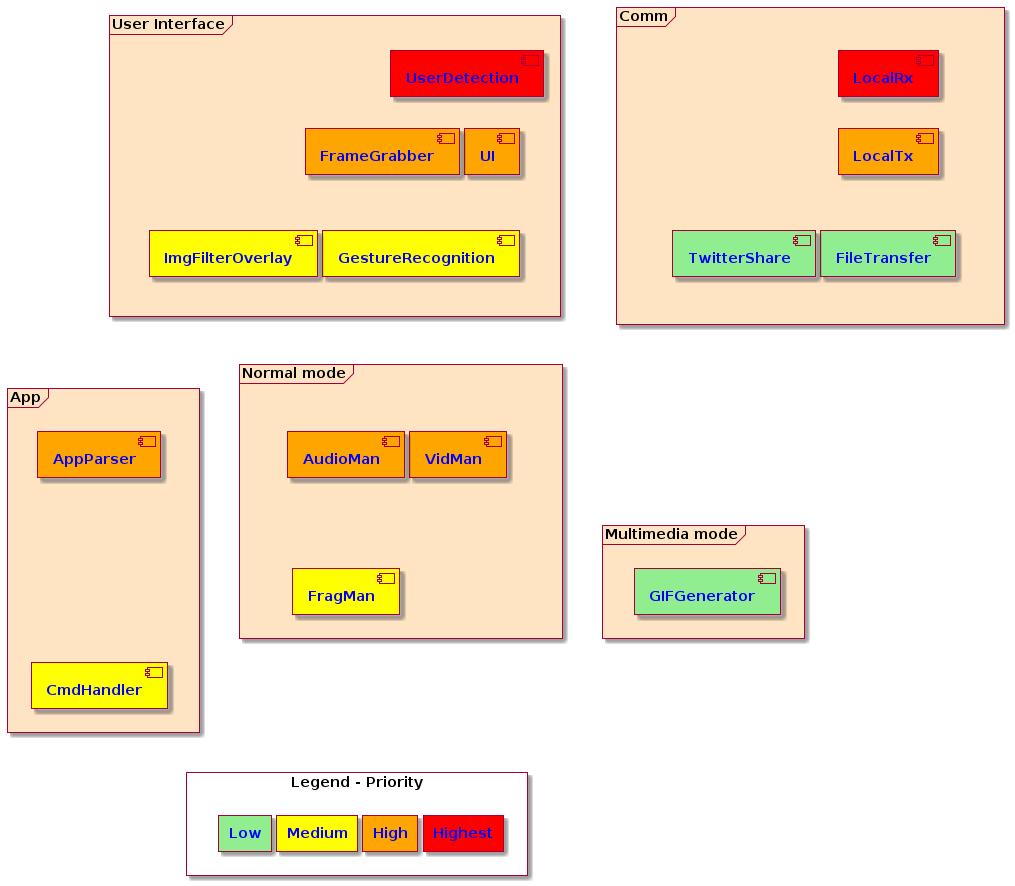
\includegraphics[width=0.8\columnwidth]{./img/thread-spec-local.png}
  \caption{Thread specification: \texttt{Local System}}%
\label{fig:thread-spec-local}
\end{figure}
%
\subsection{Flowcharts}
\label{sec:flowcharts}

In this section are presented the most important flowcharts of all the systems. 
These flowcharts are important to implement because it gives to one the essentials to build all the system.

\subsubsection{Remote Client}
\label{sec:rc-flowcharts}

In the \texttt{Remote Client} there are several functions to implement.
However, most of them have particularly the same implementation method.
This is because the class diagrams are designed in order to replicate most of the code and to have many things in common, turning everything more easy to implement and to execute.

In Fig.~\ref{fig:flow-rc-login} is the flowchart of the \texttt{Login} feature.
After the login button being pressed, it is necessary to verify if all fields are filled. If so, the password is encrypted in order to compare with the passwords from the database (that are all encrypted).
It is made a \texttt{query} to the users database to select a count and the role of all users that have the same username and password.
If the count is equal to one, then the user has its credentials validated and it is shown the view according to its role. If not, then there's an error in the login.
%
\begin{figure}[htb!]
\centering
    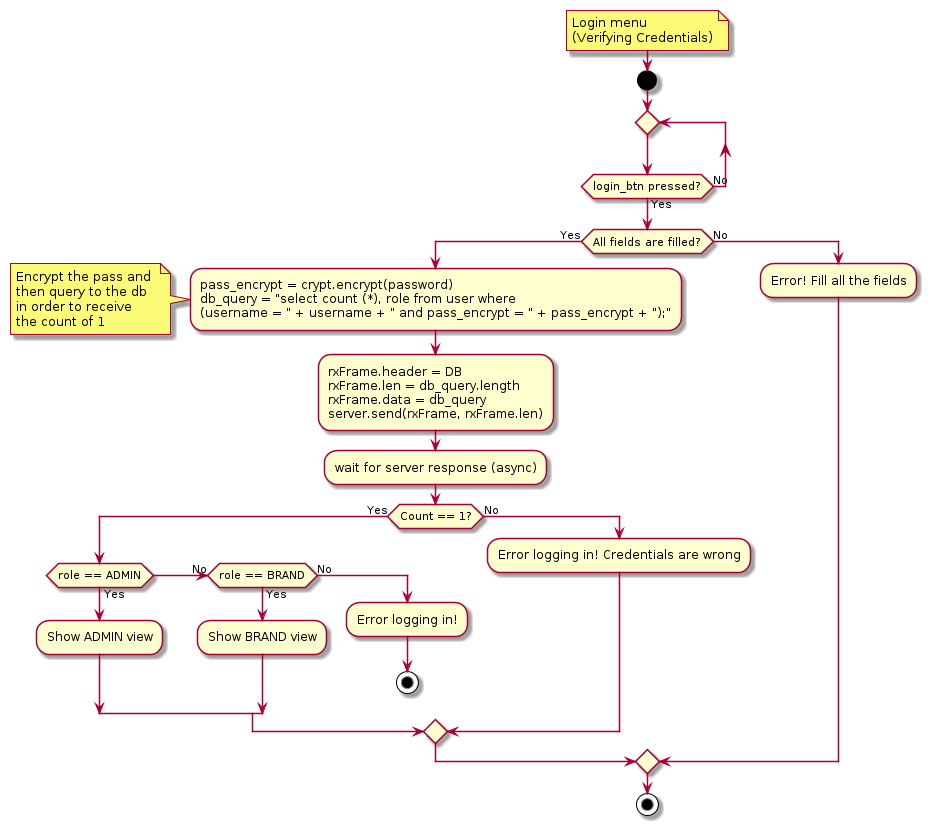
\includegraphics[width=0.8\columnwidth]{./img/flow-rc-login.png}
  \caption{Flowchart: \texttt{Remote Client} --- Login}%
\label{fig:flow-rc-login}
\end{figure}

In Fig.~\ref{fig:flow-rc-register-user} is depicted the flowchart for registering a user.
Basically, after the button being pressed and all the fields are filled, an user object is created. To know if the user can be created, it is made a \texttt{query} to the Users database to know if there is already an user with that username or that password. If not, then it is made another \texttt{query} to add that user to the users database and the registration is complete. 
%
\begin{figure}[htb!]
\centering
    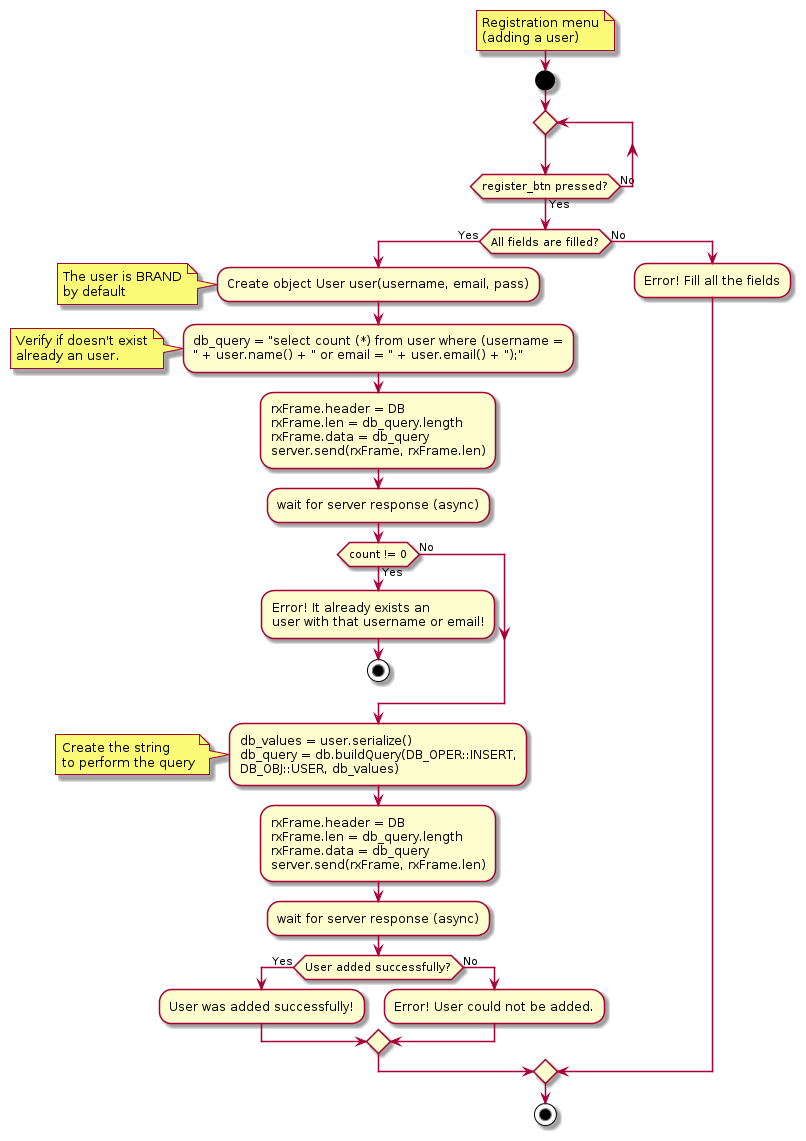
\includegraphics[width=0.8\columnwidth]{./img/flow-rc-register-user.png}
  \caption{Flowchart: \texttt{Remote Client} --- Register}%
\label{fig:flow-rc-register-user}
\end{figure}

In Fig.~\ref{fig:flow-rc-delete-user} is depicted a flowchart of the delete user feature.
Basically, the user is deleted using its id, and for that it is made a \texttt{query} to the users database to delete the row with that user id. After that query, the delete process is completed
%
\begin{figure}[htb!]
\centering
    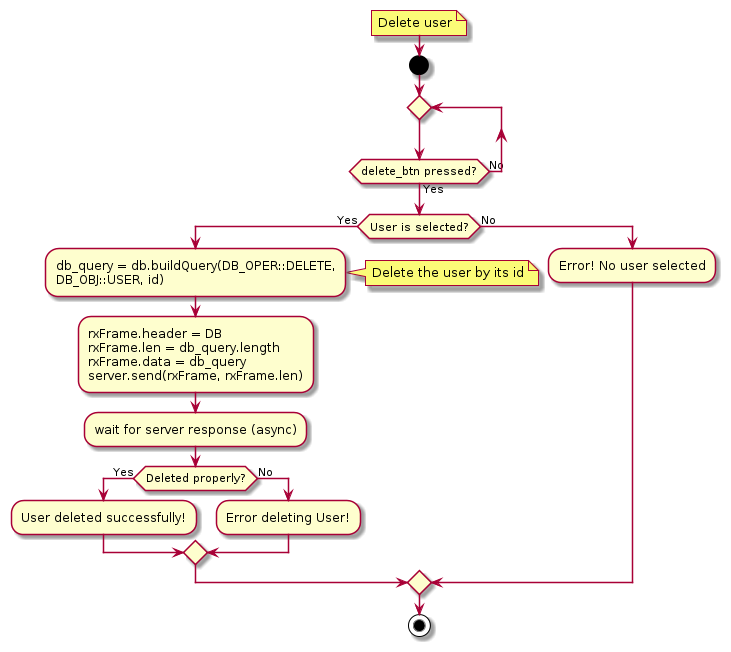
\includegraphics[width=0.8\columnwidth]{./img/flow-rc-delete-user.png}
  \caption{Flowchart: \texttt{Remote Client} --- Delete User}%
\label{fig:flow-rc-delete-user}
\end{figure}

In Fig.~\ref{fig:flow-rc-rent-ad} is the flowchart of how it behaves the rent ad feature.
Basically an ad object is created and added to the timetable object. After that, it is made a \texttt{query} to the time table database to add the ad to the specific time slots. Then, if everything occurs as expected, the Ad is then added to the database by a \texttt{query}. If that query don't occur as expected, then the timetable previously added needs to be removed from the database.
%
\begin{figure}[htb!]
\centering
    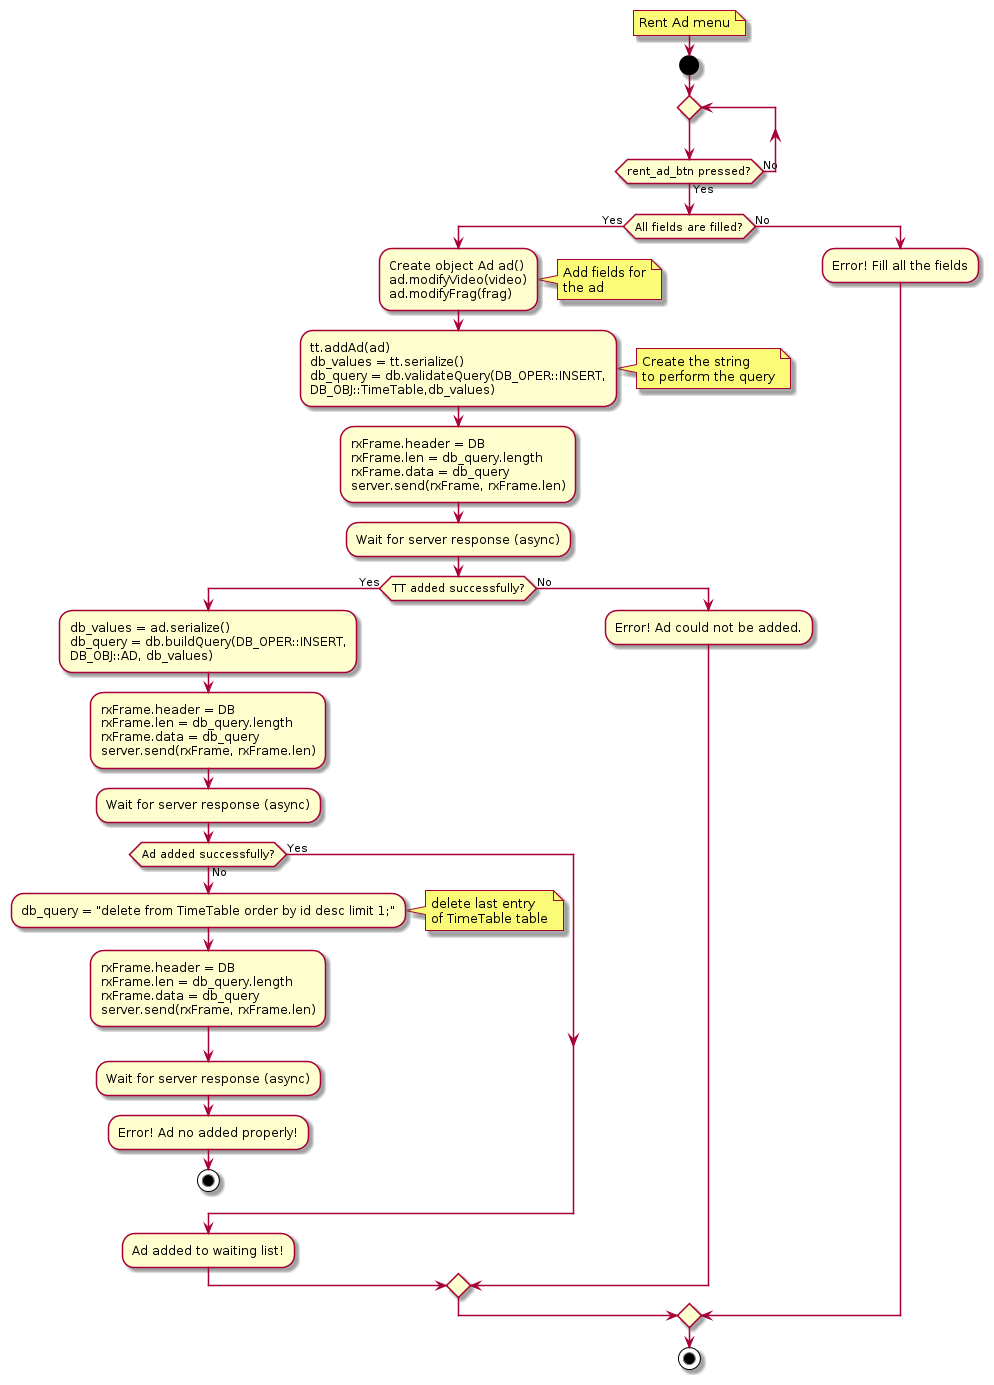
\includegraphics[width=0.8\columnwidth]{./img/flow-rc-rent-ad.png}
  \caption{Flowchart: \texttt{Remote Client} --- Rent Ad}%
\label{fig:flow-rc-rent-ad}
\end{figure}

\subsubsection{Remote Server}
\label{sec:rs-flowcharts}
%
The \texttt{Remote Server} is the connection node between the \texttt{Remote Client} and the \texttt{Local System}. Also, it has an important influence in the databases. So, there are several functions to implement.
The most important functions to implement are the thread functions. Some of them can be analogous which can be good because most of the code can be replicated.

Fig.~\ref{fig:flow-rs-recv} shows how the receive thread is implemented.
Basically this thread waits to receive data from a socket and after that, add that received command to the vector RxVec. In this situation it is mandatory to use mutexes to avoid accessing RxVec at the same time in different threads. Also it is used a semaphore to handle the number of threads that can use this vector.
The send thread is particularly the same thing, with the difference that it is necessary to know if there is something to send and send it. The information of the socket is already in the txVec and it is easy to send the information to the specific side.
%
\begin{figure}[htb!]
\centering
    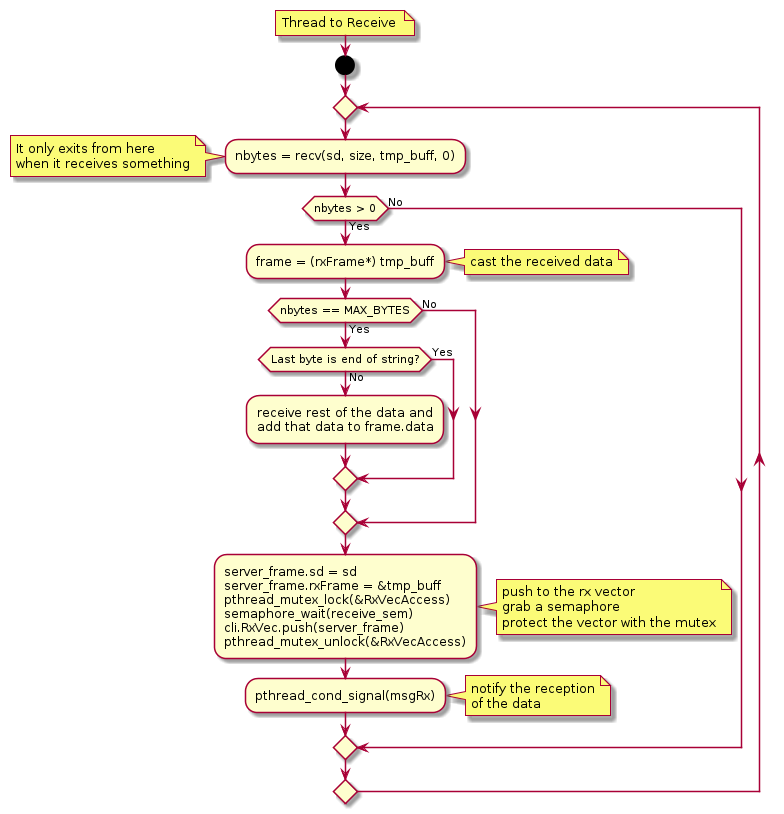
\includegraphics[width=0.7\columnwidth]{./img/flow-rs-recv.png}
  \caption{Flowchart: \texttt{Remote Server} --- Receive Thread}%
\label{fig:flow-rs-recv}
\end{figure}

Fig.~\ref{fig:flow-rs-parser} shows how the parser is executed.
Basically this thread verifies if it exists messages received to read, if so, they are popped from the \gls{fifo} and it is dropped the semaphore that was being used.
Then, by the structure rxFrame it is verified if the data is a command or a database query. If it is a command, it is signalized that it is a command and it is added to the vector, if it is a database query, it does the same but for the signal of the database handle and the db vector.
It is always mandatory to avoid collisions of data, using for that the mutexes to lock the usage of the vectors.
%
\begin{figure}[htb!]
\centering
    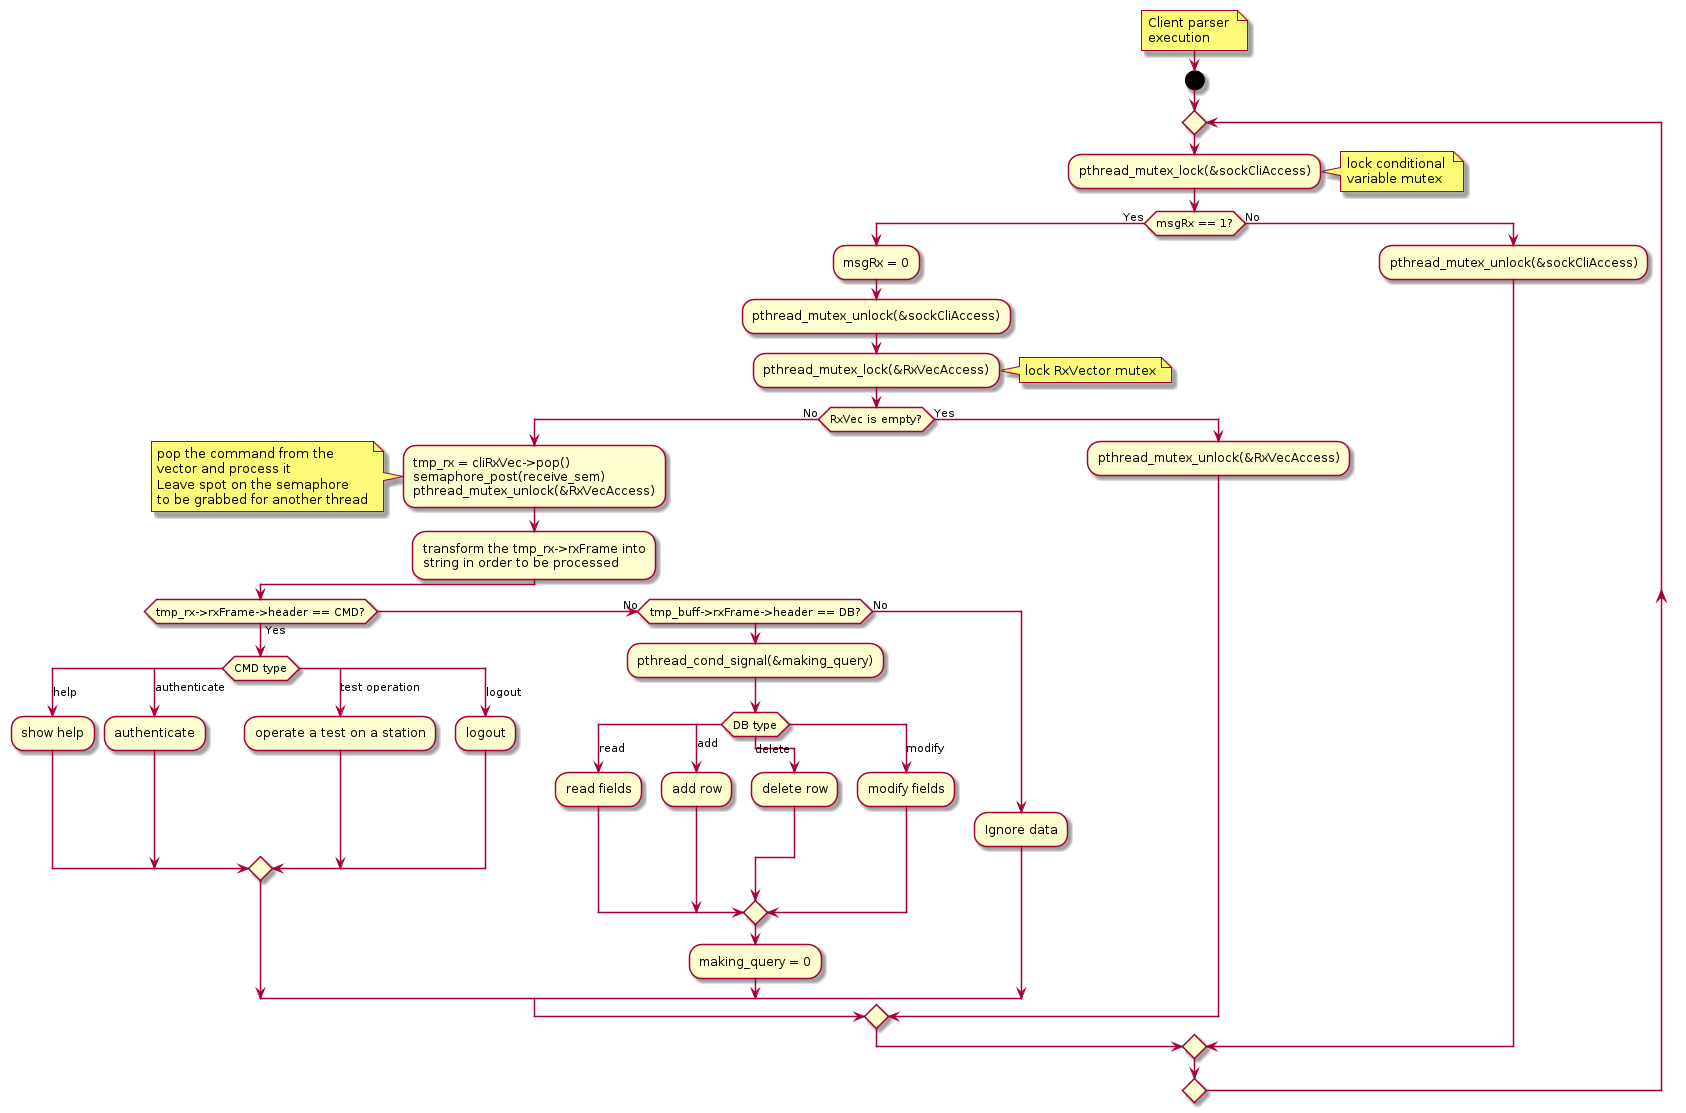
\includegraphics[width=0.8\columnwidth]{./img/flow-rs-parser.png}
  \caption{Flowchart: \texttt{Remote Server} --- Parser}%
\label{fig:flow-rs-parser}
\end{figure}

Fig.~\ref{fig:flow-rs-handle-cmd} shows how the handleCmd thread is processed.
Firstly, it is necessary to pop a command from the cmdVec and then execute it.
It is necessary to know if the command is to execute in the remote server or to send to the local system. If it is to send to the local system, it is needed to make a query to the database to know the ip of the local system and then send to the machine. 
%
\begin{figure}[htb!]
\centering
    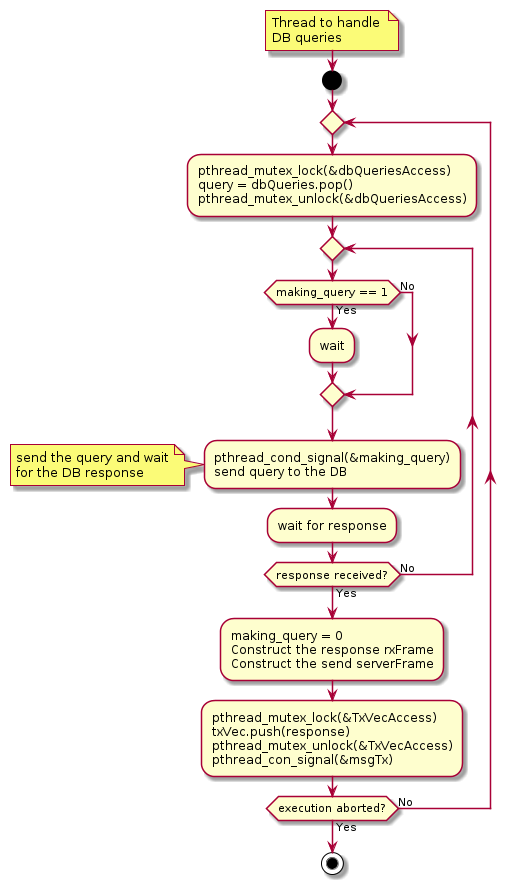
\includegraphics[width=0.4\columnwidth]{./img/flow-rs-handle-query.png}
  \caption{Flowchart: \texttt{Remote Server} --- handleQuery}%
\label{fig:flow-rs-handle-query}
\end{figure}

Fig.~\ref{fig:flow-rs-handle-query} shows how the handleQuery thread is processed.
Firstly, it is necessary to retrieve a query from the vector dbQueries (using the mutex to save the vector from other usage) and then make the query if no one is querying the database.
After the query, it is received and stored the response to then send to the other side. So, the response is saved on the TxVec that already has the destination socket.
%
\begin{figure}[htb!]
\centering
    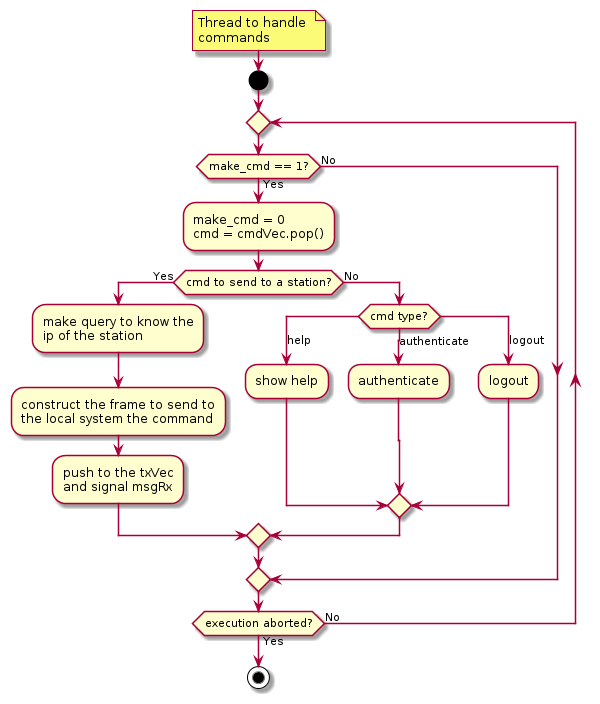
\includegraphics[width=0.4\columnwidth]{./img/flow-rs-handleCmd.png}
  \caption{Flowchart: \texttt{Remote Server} --- handleCmd}%
\label{fig:flow-rs-handle-cmd}
\end{figure}


Fig.~\ref{fig:flow-rs-update-local-sys} illustrates how the update local system works.
Basically, when some field from the database is changed and it is necessary to inform the local system to change its behavior, the database sends a trigger that is received from this thread. After that, the thread needs to make the query to the explicit database that made the trigger to ask for all the information that changed to send to the station.
After receiving the responses from the queries, everything is wrapped in the txVec (that also will contain to which station to send) and it is signaled the need to send information.
%
\begin{figure}[htb!]
\centering
    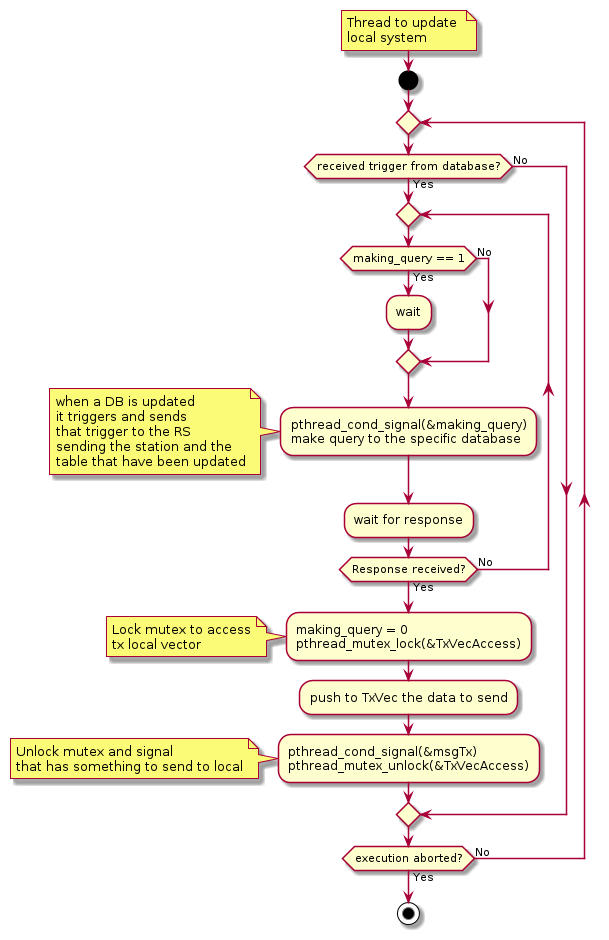
\includegraphics[width=0.6\columnwidth]{./img/flow-rs-updt-local-sys.png}
  \caption{Flowchart: \texttt{Remote Server} --- updateLocalSys}%
\label{fig:flow-rs-update-local-sys}
\end{figure}


%\section{Software interfaces definition}
%\label{sec:sw-interf-def}
%- Define the APIs in detail:
%  - header files with:
%    - functions prototypes
%    - data structure declarations
%    - class declarations
%
% From the state machine diagram (Fig.~\ref{fig:state-mach}) the softwares modules
% and data structures can be infered. The data structure is \texttt{keycode\_fifo},
% a circular buffer to manage the keycodes produced and consumed. The modules are
% \texttt{i2c}, \texttt{ir} and \texttt{fifo} for determing the key pressed,
% transmitting the keycode and managing the \gls{fifo} buffer. Enumerations are
% added for keycodes and errors listing.
% 
% An example of the \gls{api} can be seen in Listing~\ref{lst:api}, using builtin documentation.
% %
% \lstinputlisting[language=c, firstline=1,caption={\gls{api} example with
%   builtin documentation},label=lst:api,
% style=customc]{./listing/api.h}%%%%%%%%%%%%%%%%%%%%
%
%\section{Start-up/shutdown process specification}
%\label{sec:startup-shutdown}
%As highlighted in Fig.~\ref{fig:state-mach}, the process starts with battery
%power being supplied to the system, going into sleep mode and waiting for
%events, minimizing power consumption. However, there is still residual power
%being drawn. This could be overcome by placing a power button for the remote
%itself, but with the inconvenience of MCU reset and the initial delays
%associated. The shutdown results from batteries disconnection.\%%%%%%%
%
%\section{Error handling specification}
%\label{sec:error-handling-specification}
%Every system is prone to glitches, bugs and errors, thus, requiring it to be
%handled. Errors should be handled gracefully by creating error handling
%routines, which try to circumvent them and provide feedback.
%
%For extreme cases, where this is not possible, the watchdog timer should be
%enabled to help the system recover from crashes. However, this is a last resort,
%as constant reboots --- sign of a bad design --- are inadmissible and will
%frustrate the user.
%
%The error handling routines can be built into the design by considering return
%codes and asserts from function calls, e.g., \texttt{int i2c\_read(char *byte)},
%where \texttt{0} signals success and otherwise an error was encountered. Thus,
%good design eases error-handling specification and should be an aspect to keep
%in mind in this phase.
%%

\subsubsection{Local System}
\label{sec:local-system-3}
Fig.~\ref{fig:flow-local-user-detect} through Fig.~\ref{fig:flow-local-gif-gen} present the flowcharts corresponding to the \texttt{Local System}
threads specified in Section~\ref{sec:local-system-2}.

\paragraph{UserDetection thread}
Fig.~\ref{fig:flow-local-user-detect} depicts the flowchart for the
\texttt{UserDetection} thread. It is executed periodically to check if an
\texttt{User} was detected, consuming user detection events from a message
queue that the ultrasonic sensor daemon must update.

If an \texttt{User} was detected, then the current value is added to a sliding
window to determine if its a valid user detection. If the user was detected,
this event is signaled.
%
\begin{figure}[htb!]
\centering
    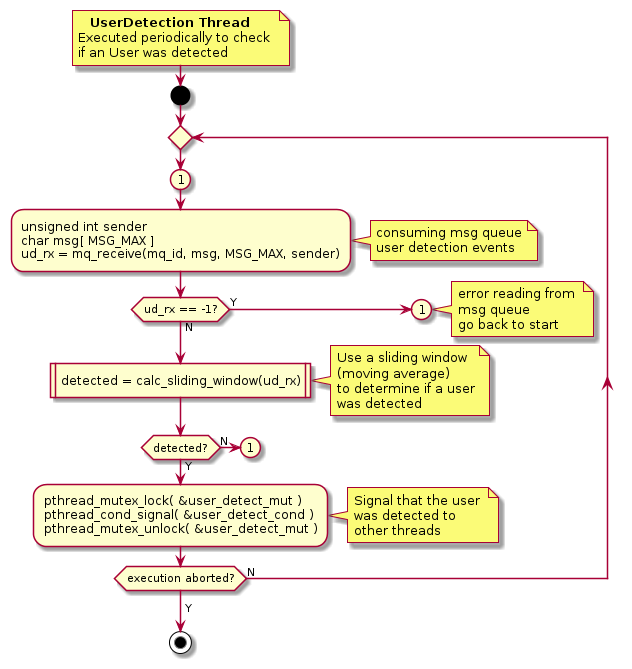
\includegraphics[width=0.6\columnwidth]{./img/flow-local-user-detect.png}
  \caption{Flowchart: \texttt{Local System} --- \texttt{UserDetect} thread}%
\label{fig:flow-local-user-detect}
\end{figure}
%
\paragraph{FrameGrabber thread}
Fig.~\ref{fig:flow-local-frame-grabber} depicts the flowchart for the
\texttt{FrameGrabber} thread. It is executed periodically, accordingly to the
frame rate defined, to grab frames from camera and store them. It produces
camera frames that are stored into a shared \gls{fifo} and it uses a semaphore
to handle multiple consumer threads access.
%
\begin{figure}[htb!]
\centering
    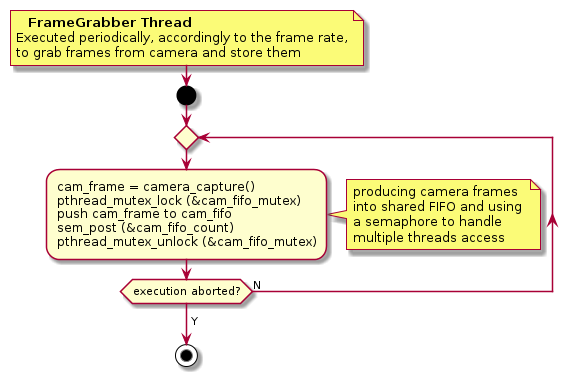
\includegraphics[width=0.6\columnwidth]{./img/flow-local-frame-grabber.png}
  \caption{Flowchart: \texttt{Local System} --- \texttt{FrameGrabber} thread}%
\label{fig:flow-local-frame-grabber}
\end{figure}
%
\paragraph{LocalRx thread}
Fig.~\ref{fig:flow-local-rx} depicts the flowchart for the \texttt{LocalRx}
thread. It is listening on the socket used to communicate with the
\texttt{Remote Server} for incoming data packets. When data arrives, it is
validated by checking for the \texttt{ACK} signal. If the frame is correct and
terminated it is pushed to a shared \gls{fifo} and this event is signaled for
the consuming thread --- \texttt{AppParser}.
%
\begin{figure}[htb!]
\centering
    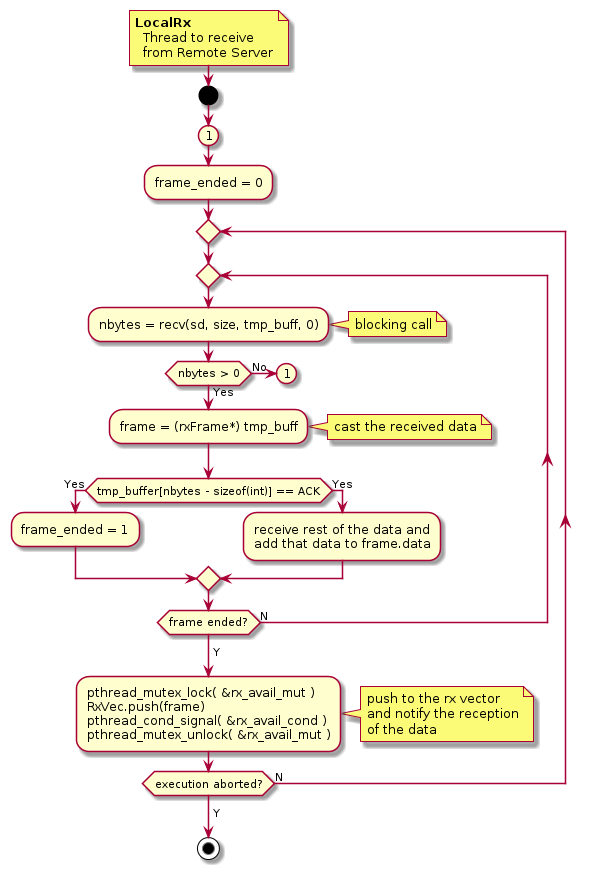
\includegraphics[width=0.6\columnwidth]{./img/flow-local-rx.png}
  \caption{Flowchart: \texttt{Local System} --- \texttt{LocalRx} thread}%
\label{fig:flow-local-rx}
\end{figure}
\paragraph{LocalTx thread}
Fig.~\ref{fig:flow-local-tx} depicts the flowchart for the \texttt{LocalTx}
thread. It waits for data to be transmitted to become available, pops it from
the shared \gls{fifo} and sends it to the \texttt{Remote Server}.
%
\begin{figure}[htb!]
\centering
    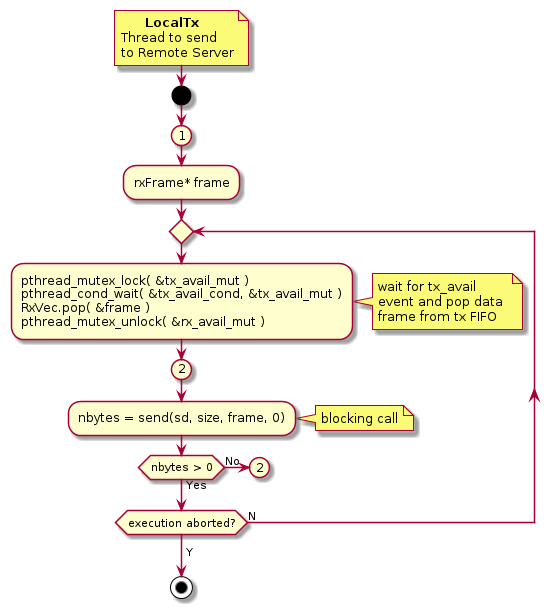
\includegraphics[width=0.6\columnwidth]{./img/flow-local-tx.png}
  \caption{Flowchart: \texttt{Local System} --- \texttt{LocalTx} thread}%
\label{fig:flow-local-tx}
\end{figure}
%
\paragraph{AppParser thread}
Fig.~\ref{fig:flow-local-app-parser} depicts the flowchart for the \texttt{AppParser}
thread.
It waits for received data to become available, and then processes all frames in
that shared \gls{fifo}.
It has two main flows, depending on the frame header. If it is a command the
data is casted to a \texttt{cmdFrame}, pushed to a shared buffer and this event
is signaled for the \texttt{CmdHandler} thread to process these data. If it is
an \texttt{Ad}, the data is casted to a \texttt{adFrame}, pushed to a shared
buffer and this event is signaled to the \texttt{FileTransfer} thread so it can
download media files.
%
\begin{figure}[htb!]
\centering
    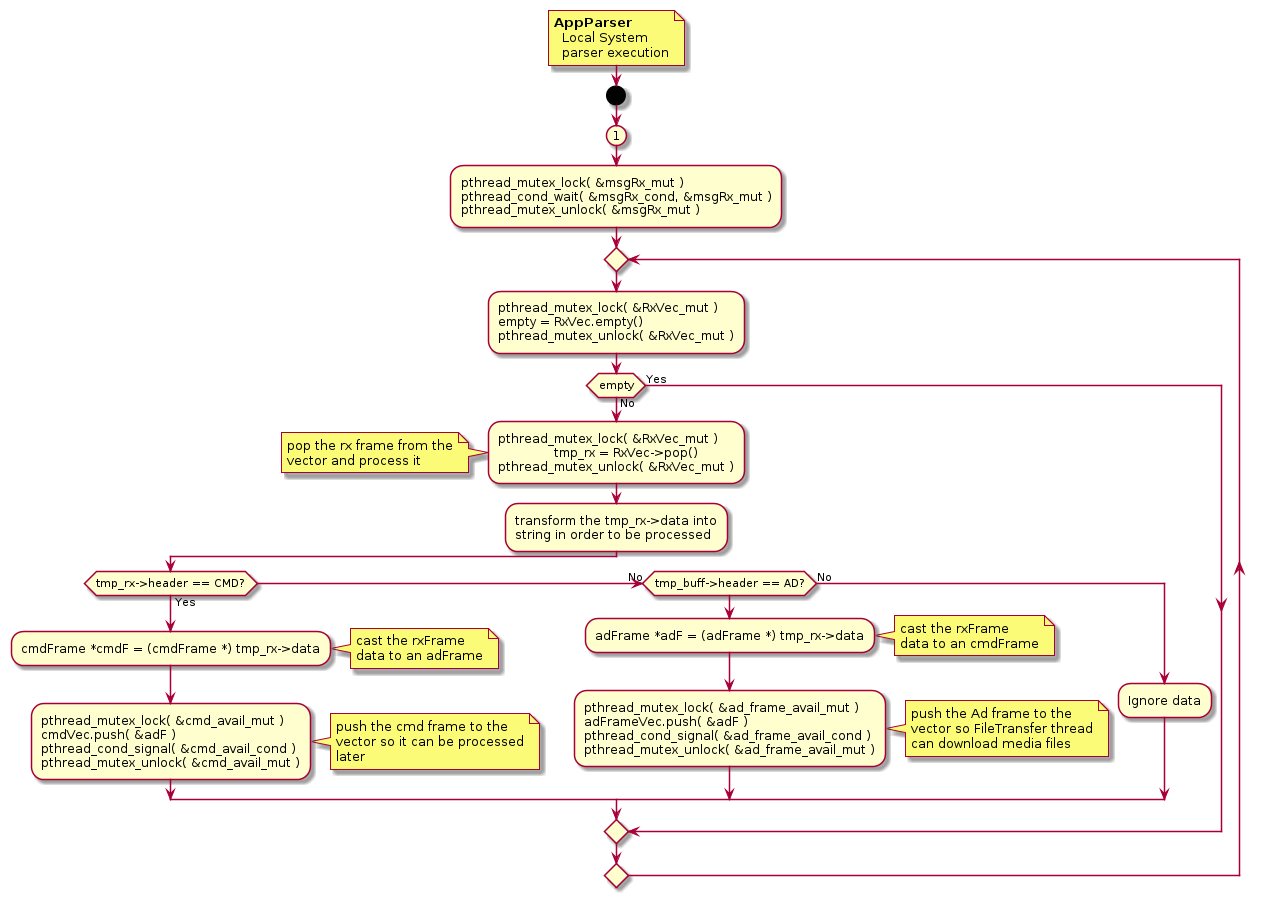
\includegraphics[width=1.0\columnwidth]{./img/flow-local-app-parser.png}
  \caption{Flowchart: \texttt{Local System} --- \texttt{AppParser} thread}%
\label{fig:flow-local-app-parser}
\end{figure}
% 
\paragraph{CmdHandler thread}
Fig.~\ref{fig:flow-local-cmd-handler} depicts the flowchart for the
\texttt{CmdHandler} thread. It waits for commands to be available, and then
processes all commands in that shared \gls{fifo}.
%
\begin{figure}[htb!]
\centering
    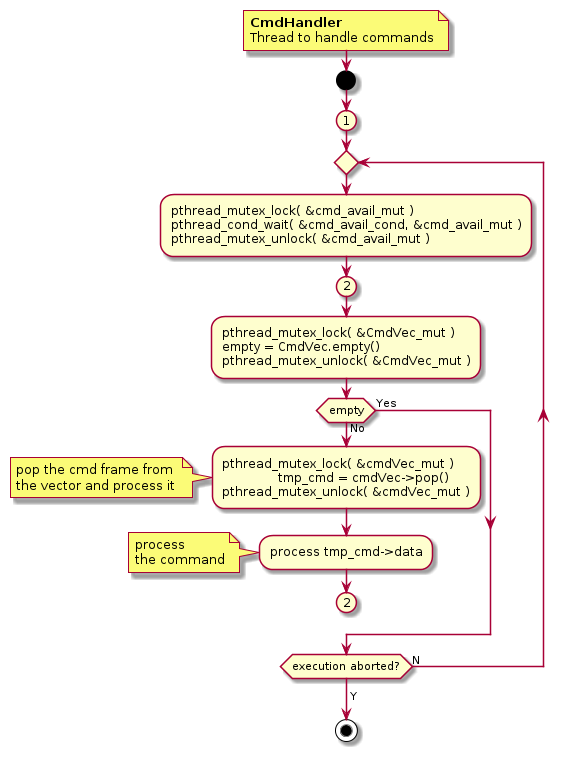
\includegraphics[width=0.55\columnwidth]{./img/flow-local-cmd-handler.png}
  \caption{Flowchart: \texttt{Local System} --- \texttt{CmdHandler} thread}%
\label{fig:flow-local-cmd-handler}
\end{figure}
\paragraph{TwitterShare thread}
Fig.~\ref{fig:flow-local-twitter-share} depicts the flowchart for the
\texttt{TwitterShare} thread. It waits for a post to be available, and then
shares it on \texttt{Twitter} --- using \texttt{curl} and \texttt{HTTP POST}
method under the hood. The share status is then updated and a signal is emitted
to the waiting thread --- \texttt{UI} --- to provide appropriate feedback to the
\texttt{User}.
%
\begin{figure}[htb!]
\centering
    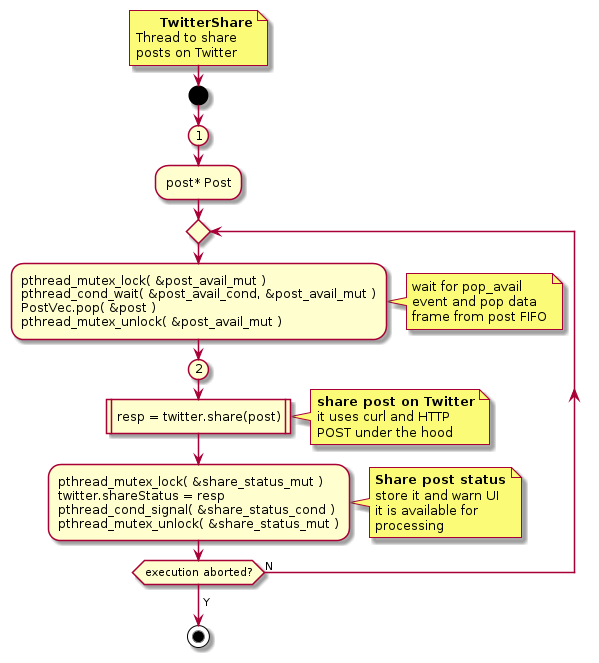
\includegraphics[width=0.6\columnwidth]{./img/flow-local-twitter-share.png}
  \caption{Flowchart: \texttt{Local System} --- \texttt{TwitterShare} thread}%
\label{fig:flow-local-twitter-share}
\end{figure}
%
\paragraph{FileTransfer thread}
Fig.~\ref{fig:flow-local-file-transfer} depicts the flowchart for the
\texttt{FileTransfer} thread. It waits for \texttt{Ad} frame data to be
available and then pops it. It constructs a new \texttt{Ad} object. It then
retrieves the \gls{csv} string \texttt{mediaURLs} and tokenizes it, using the
comma as the delimiter token, to extract all \glspl{url}. While there are
\glspl{url} available, the file is downloaded from the \gls{url} proxy server
and the filename is stored in a \gls{fifo} for later reference.
%
\begin{figure}[htb!]
\centering
    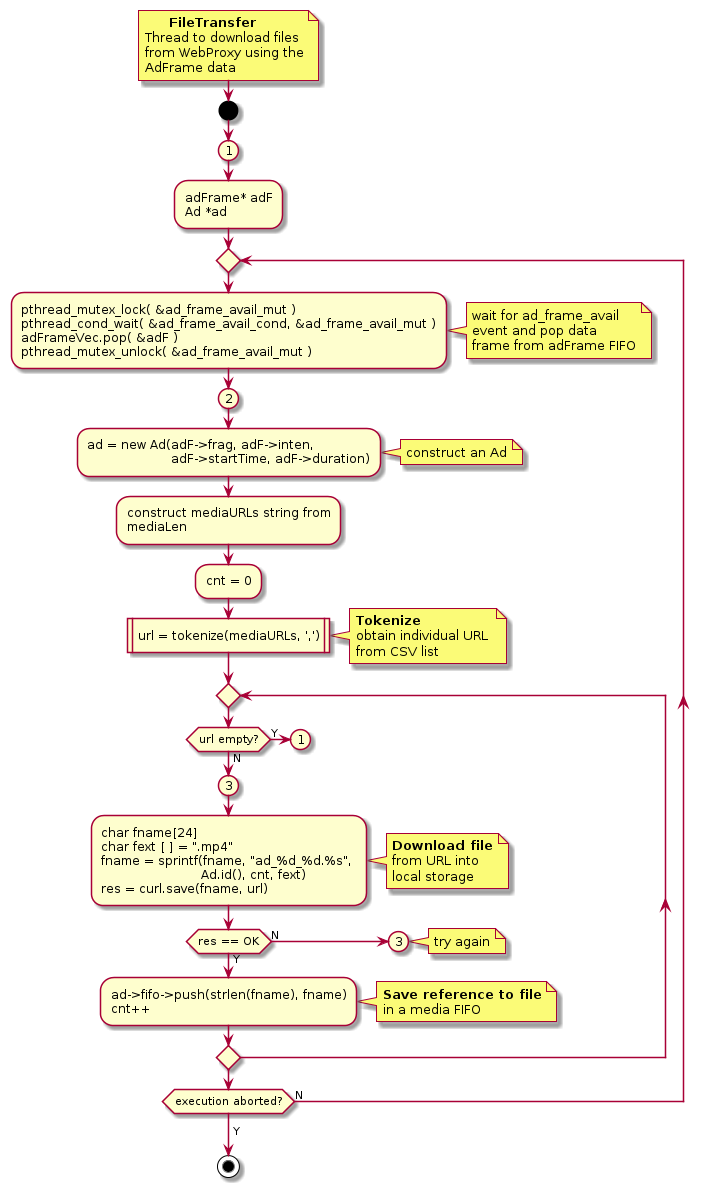
\includegraphics[width=0.6\columnwidth]{./img/flow-local-file-transfer.png}
  \caption{Flowchart: \texttt{Local System} --- \texttt{FileTransfer} thread}%
\label{fig:flow-local-file-transfer}
\end{figure}
%
\begin{figure}[htb!]
\centering
    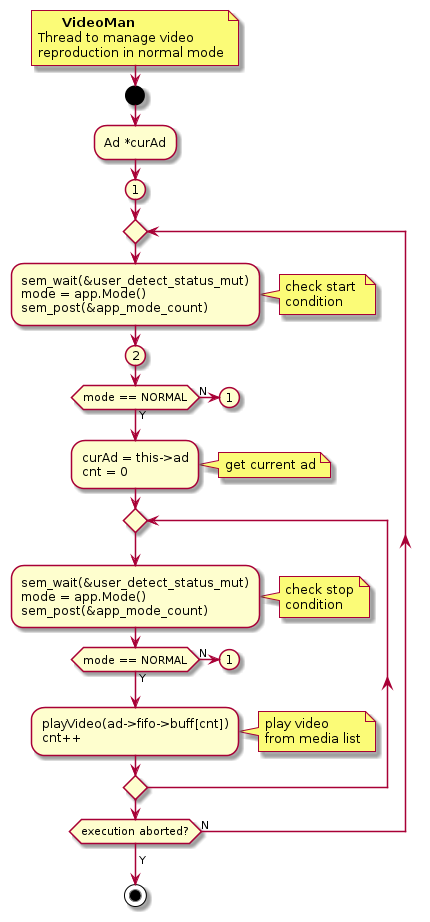
\includegraphics[width=0.6\columnwidth]{./img/flow-local-video-man.png}
  \caption{Flowchart: \texttt{Local System} --- \texttt{VidMan} thread}%
\label{fig:flow-local-video-man}
\end{figure}
%
\begin{figure}[htb!]
\centering
    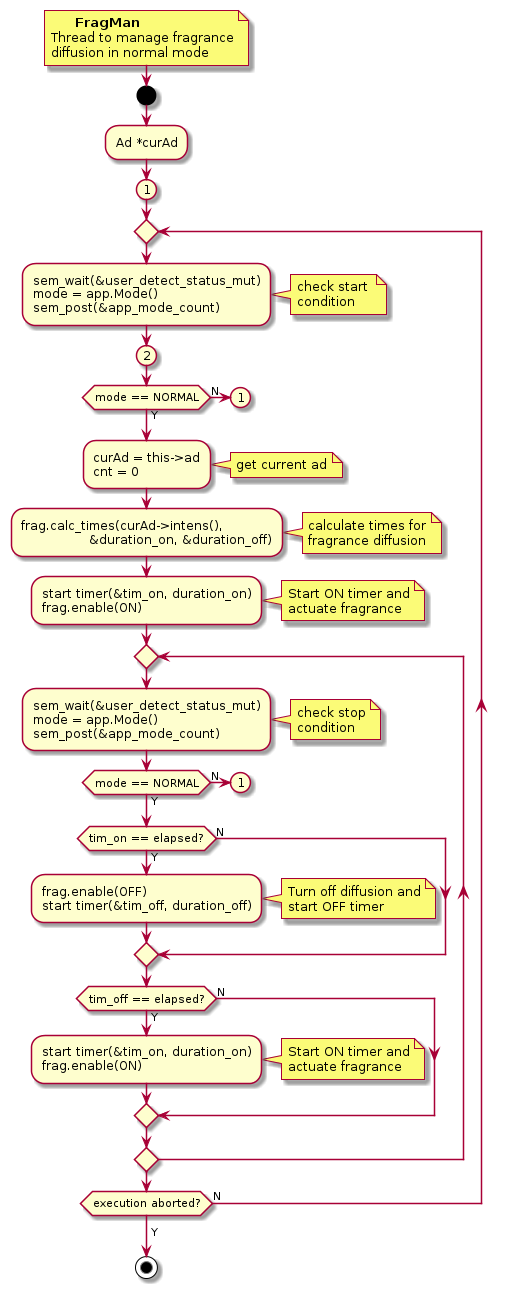
\includegraphics[width=0.6\columnwidth]{./img/flow-local-frag-man.png}
  \caption{Flowchart: \texttt{Local System} --- \texttt{FragMan} thread}%
\label{fig:flow-local-frag-man}
\end{figure}
%
\begin{figure}[htb!]
\centering
    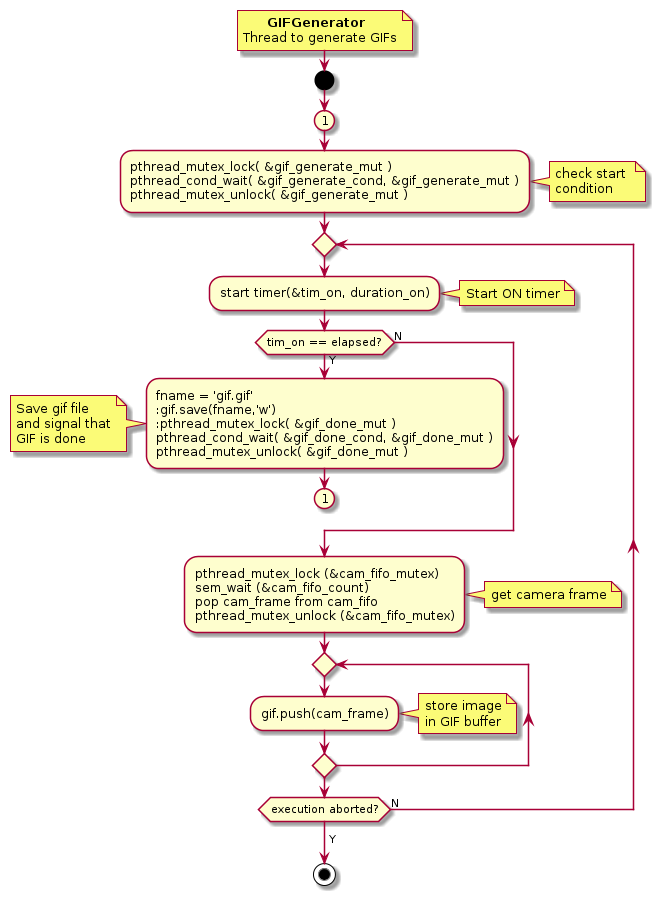
\includegraphics[width=0.6\columnwidth]{./img/flow-local-gif-gen.png}
  \caption{Flowchart: \texttt{Local System} --- \texttt{GIFGenerator} thread}%
\label{fig:flow-local-gif-gen}
\end{figure}


\subsection{Test cases}
\label{sec:sw-test-cases}
In order to verify if all the software is in good conditions, are made some functional test cases to each subsystem to see if the results combine with the expected ones.

\subsubsection{Remote Client}
\label{sec:test-cases-rc}
In table \ref{tab:test-cases-rc} is depicted the test cases for the \texttt{Remote Client}. These test cases are mostly made through the UI verifying if this is responding as it should. Examples can be seen in the table, such as \texttt{Register}, \texttt{Login}, \texttt{Logout} and so on.
%
\begingroup
\renewcommand{\arraystretch}{0.7} % Default value: 1
% Please add the following required packages to your document preamble:
% \usepackage{booktabs}
\begin{table}[]
\centering
\caption{Remote Client Test Cases}
\label{tab:test-cases-rc}
\begin{tabular}{@{}llll@{}}
\toprule
\textbf{Use Case}                                              & \textbf{Type of test} & \textbf{Description}                                                                                                               & \textbf{Expected Result}                                                                                                                       \\ \midrule
Register                                                       & Functional            & \begin{tabular}[c]{@{}l@{}}One will try to make a new register\\ as a Brand\end{tabular}                                           & \begin{tabular}[c]{@{}l@{}}If the User is created and added to\\ the database, everything is in order\end{tabular}                             \\ \midrule
Login                                                          & Functional            & \begin{tabular}[c]{@{}l@{}}One will try to Login through its user\\ and password.\end{tabular}                                     & \begin{tabular}[c]{@{}l@{}}If the login is successful, everything\\ is working as expected.\end{tabular}                                       \\ \midrule
Logout                                                         & Functional            & One will try to log out from the account.                                                                                          & If it returns to the login page, it works.                                                                                                     \\ \midrule
\begin{tabular}[c]{@{}l@{}}Manage\\ User\end{tabular}          & Functional            & \begin{tabular}[c]{@{}l@{}}One will manage a user removing it or \\ giving him privileges as Admin.\end{tabular}                   & \begin{tabular}[c]{@{}l@{}}If the user is removed from the DB or\\ has privileges as admin, it works well.\end{tabular}                        \\ \midrule
\begin{tabular}[c]{@{}l@{}}Manage\\ Station\end{tabular}       & Functional            & \begin{tabular}[c]{@{}l@{}}One will try to manage a station by\\ powering on/off, manage ads or enable/\\ disable ad.\end{tabular} & \begin{tabular}[c]{@{}l@{}}If the information is updated and \\ the station reacts to the commands,\\ the system is working well.\end{tabular} \\ \midrule
\begin{tabular}[c]{@{}l@{}}Test\\ Operation\end{tabular}       & Functional            & \begin{tabular}[c]{@{}l@{}}One will choose to test the operation\\ of the machine.\end{tabular}                                    & \begin{tabular}[c]{@{}l@{}}If a command line is provided with the\\ remote server, it works properly.\end{tabular}                             \\ \midrule
\begin{tabular}[c]{@{}l@{}}Display\\ Rented\\ Ads\end{tabular} & Functional            & \begin{tabular}[c]{@{}l@{}}One will try to display the rented ads\\ by the user in case.\end{tabular}                              & \begin{tabular}[c]{@{}l@{}}If there are displayed all the ads of\\ that brand, then everything works\\ properly.\end{tabular}                  \\ \midrule
Rent Ads                                                       & Functional            & \begin{tabular}[c]{@{}l@{}}One will try to rent ads as a brand,\\ inserting all data necessary.\end{tabular}                       & \begin{tabular}[c]{@{}l@{}}If the remote client responds in order,\\ saving all data in the DB, it works well.\end{tabular}                    \\ \midrule
\begin{tabular}[c]{@{}l@{}}See\\ Notifications\end{tabular}    & Functional            & \begin{tabular}[c]{@{}l@{}}One will try to watch the notifications\\ of a brand.\end{tabular}                                      & \begin{tabular}[c]{@{}l@{}}If the brand has notifications, it should \\ be displayed. This means that it works.\end{tabular}                   \\ \bottomrule
\end{tabular}
\end{table}

\subsubsection{Remote Server}
\label{test-cases-rs}
In table \ref{tab:test-cases-rs} are illustrated the test cases for the \texttt{Remote Server}. Theses tests are divided in two parts: the part that belongs to the server parsing and execution commands and the part that belongs to send commands to the stations in order to test their operation. These last kind of tests can also entry on the \texttt{Local System} test cases, because it is needed a feedback from the \gls{mdo-l}.
%
\begingroup
\renewcommand{\arraystretch}{0.7} % Default value: 1
% Please add the following required packages to your document preamble:
% \usepackage{booktabs}
\begin{table}[]
\centering
\caption{Remote Server Test Cases}
\label{tab:test-cases-rs}
\begin{tabular}{@{}llll@{}}
\toprule
\textbf{Use Case}                                                 & \textbf{Type of test} & \textbf{Description}                                                                                                                                                              & \textbf{Expected Result}                                                                                                                                                                              \\ \midrule
Disconnect                                                        & Functional            & One will try to disconnect.                                                                                                                                                       & It has to disconnect successfully.                                                                                                                                                                    \\ \midrule
\begin{tabular}[c]{@{}l@{}}Authenticate\\ User\end{tabular}       & Functional            & \begin{tabular}[c]{@{}l@{}}One will try to authenticate a user\\ already present in the database.\end{tabular}                                                                    & \begin{tabular}[c]{@{}l@{}}The server needs to respond in order:\\ accept authentication or decline if failed.\end{tabular}                                                                           \\ \midrule
Help                                                              & Functional            & One will try to get help.                                                                                                                                                         & \begin{tabular}[c]{@{}l@{}}Information to help the user should be \\ provided.\end{tabular}                                                                                                           \\ \midrule
\begin{tabular}[c]{@{}l@{}}Interact with\\ databases\end{tabular} & Functional            & \begin{tabular}[c]{@{}l@{}}One will try to query a database, reading,\\ modifying, adding or deleting something.\end{tabular}                                                     & \begin{tabular}[c]{@{}l@{}}If the database is correctly updated\\ according to the command, then it works.\end{tabular}                                                                               \\ \midrule
\multicolumn{4}{c}{\textbf{Test Operation}}                                                                                                                                                                                                                                                                                                                                                                                                                                           \\ \midrule
\begin{tabular}[c]{@{}l@{}}Manage\\ User\end{tabular}             & Functional            & \begin{tabular}[c]{@{}l@{}}One will manage a user removing it or \\ giving him privileges as Admin.\end{tabular}                                                                  & \begin{tabular}[c]{@{}l@{}}If the user is removed from the DB or\\ has privileges as admin, it works well.\end{tabular}                                                                               \\ \midrule
\begin{tabular}[c]{@{}l@{}}Manage\\ Audio\end{tabular}            & Functional            & \begin{tabular}[c]{@{}l@{}}One will try to manage the audio, \\ playing an audio file that is present\\ on the database.\end{tabular}                                             & \begin{tabular}[c]{@{}l@{}}The server must send the information of\\ the audio to play to the local system. If\\ it works, then it is verified.\end{tabular}                                          \\ \midrule
\begin{tabular}[c]{@{}l@{}}Manage\\ Video\end{tabular}            & Functional            & \begin{tabular}[c]{@{}l@{}}One will try to manage the video, \\ playing a video file that is present\\ on the database.\end{tabular}                                              & \begin{tabular}[c]{@{}l@{}}The server must send the information of\\ the video to play to the local system. If\\ it works, then it is verified.\end{tabular}                                          \\ \midrule
\begin{tabular}[c]{@{}l@{}}Manage\\ Fragrance\end{tabular}        & Functional            & \begin{tabular}[c]{@{}l@{}}One will try to activate a fragrance\\ diffusion to the machine.\end{tabular}                                                                          & \begin{tabular}[c]{@{}l@{}}If the server sends the right information\\ to the LS, then the LS should diffuse the\\ fragrance.\end{tabular}                                                            \\ \midrule
\begin{tabular}[c]{@{}l@{}}Manage\\ Camera\end{tabular}           & Functional            & \begin{tabular}[c]{@{}l@{}}One will try to manage the camera\\ with its various features (turn on/off,\\ facial recognition, take GIF, take picture\\ apply filter).\end{tabular} & \begin{tabular}[c]{@{}l@{}}If the remote server sends the right info,\\ then the local system should actuate in \\ the camera according to the function that\\ was requested to operate.\end{tabular} \\ \midrule
Share                                                             & Functional            & \begin{tabular}[c]{@{}l@{}}One will try to share some file through\\ social media.\end{tabular}                                                                                   & \begin{tabular}[c]{@{}l@{}}If the LS responds correctly to that \\ command, then it is working properly.\end{tabular}                                                                                 \\ \bottomrule
\end{tabular}
\end{table}

\subsubsection{Local System}
\label{test-cases-ls}
In table \ref{tab:test-cases-ls} are depicted the test cases for the \texttt{Local System}. These test are functional and have as purpose to know if the machine is working well, if the ads are being played, if the face is being well detected and so on. Basically, it is a test operation to all functionalities of the machine.
%
\begingroup
\renewcommand{\arraystretch}{0.7} % Default value: 1
%
% Please add the following required packages to your document preamble:
% \usepackage{booktabs}
\begin{table}[]
\centering
\caption{Local System Test Cases}
\label{tab:test-cases-ls}
\begin{tabular}{@{}llll@{}}
\toprule
\textbf{Use Case}                                                & \textbf{Type of test} & \textbf{Description}                                                                                                 & \textbf{Expected Result}                                                                                                                                                           \\ \midrule
\begin{tabular}[c]{@{}l@{}}Establish\\ Connection\end{tabular}   & Functional            & \begin{tabular}[c]{@{}l@{}}One will try to establish connection to\\ the machine\end{tabular}                        & \begin{tabular}[c]{@{}l@{}}If the connection is established and the\\ credentials are verified, everything works.\end{tabular}                                                     \\ \midrule
\begin{tabular}[c]{@{}l@{}}End remote\\ Connection\end{tabular}  & Functional            & \begin{tabular}[c]{@{}l@{}}One will try to end the remote \\ connection.\end{tabular}                                & \begin{tabular}[c]{@{}l@{}}If the connection is ended correctly, then it\\ works as expected.\end{tabular}                                                                         \\ \midrule
\begin{tabular}[c]{@{}l@{}}Select Image\\ Filter\end{tabular}    & Functional            & \begin{tabular}[c]{@{}l@{}}One will try to select an image filter \\ and use it.\end{tabular}                        & \begin{tabular}[c]{@{}l@{}}It has to apply correctly the facial detection\\ and also apply correctly the filter.\end{tabular}                                                      \\ \midrule
Take Picture                                                     & Functional            & One will try to take a picture.                                                                                      & \begin{tabular}[c]{@{}l@{}}The Local System has to take the picture \\ and store it in order to behave properly.\end{tabular}                                                      \\ \midrule
Create GIF                                                       & Functional            & One will try to create a GIF.                                                                                        & \begin{tabular}[c]{@{}l@{}}The Local System has to generate the GIF \\ and store it in order to work properly.\end{tabular}                                                        \\ \midrule
\begin{tabular}[c]{@{}l@{}}Share on\\ social media\end{tabular}  & Functional            & \begin{tabular}[c]{@{}l@{}}One will try to share a picture or a \\ GIF on social media.\end{tabular}                 & \begin{tabular}[c]{@{}l@{}}If the Local System shares to the social \\ media the picture or the GIF, it works.\end{tabular}                                                        \\ \midrule
\begin{tabular}[c]{@{}l@{}}Diffuse\\ Fragrance\end{tabular}      & Functional            & One will try to diffuse the fragrance.                                                                               & If the fragrance is diffused, it works.                                                                                                                                            \\ \midrule
Play Video                                                       & Functional            & \begin{tabular}[c]{@{}l@{}}One will try to play one video of an ad\\ or something else.\end{tabular}                 & \begin{tabular}[c]{@{}l@{}}If the video plays properly, then the machine\\ is working as predicted.\end{tabular}                                                                   \\ \midrule
Play Audio                                                       & Functional            & One will try to play a random audio.                                                                                 & \begin{tabular}[c]{@{}l@{}}If the video audio plays properly, then the\\ machine is working as predicted.\end{tabular}                                                             \\ \midrule
\begin{tabular}[c]{@{}l@{}}Process\\ Commands\end{tabular}       & Functional            & \begin{tabular}[c]{@{}l@{}}One will try to send some commands \\ for the machine to process.\end{tabular}            & \begin{tabular}[c]{@{}l@{}}If the machine receives the commands \\ properly and processes them, then it \\ works well.\end{tabular}                                                \\ \midrule
Detect Face                                                      & Functional            & \begin{tabular}[c]{@{}l@{}}One will trigger the machine to detect\\ the face of a user.\end{tabular}                 & \begin{tabular}[c]{@{}l@{}}The face will be detected if the machine is\\ working properly.\end{tabular}                                                                            \\ \midrule
\begin{tabular}[c]{@{}l@{}}Recognize\\ Gesture\end{tabular}      & Functional            & \begin{tabular}[c]{@{}l@{}}One will make gestures to the camera\\ in order to see the machine behavior.\end{tabular} & \begin{tabular}[c]{@{}l@{}}The machine will recognize the gestures and\\ act according to the gesture made.\end{tabular}                                                           \\ \midrule
\begin{tabular}[c]{@{}l@{}}Update\\ Internal \\ DBs\end{tabular} & Functional            & \begin{tabular}[c]{@{}l@{}}One will try to play an ad or diffuse a\\ fragrance one more time.\end{tabular}           & \begin{tabular}[c]{@{}l@{}}The machine should update the number of\\ times the ad was played or the percentage\\ of fragrance that is still in the slot (in the DBs).\end{tabular} \\ \bottomrule
\end{tabular}
\end{table}

\subsection{\gls{cots} & third-party libraries}
\label{sec:cots}
For this project there are used several tools and libraries that are open source and help ones to develop all the subsystems. 
The tools are:
\begin{enum-c}
\item \emph{Plantuml}: draw UML diagrams
\item \emph{Make}: and makefiles
\item \emph{Doxygen}: source-code documentation
\item \emph{Qt}: UI Framework
\item \emph{Buildroot}
\item \emph{Linux}
\end{enum-c}

The third-party libraries used are:
\begin{enum-c}
\item \emph{OpenCV}: computer vision
\item \emph{Magick++}: GIF generation
\item \emph{MySQL}: DB management
\item \emph{Twitter REST APIs}
\item \emph{Curlpp + Transfer.sh}: file transfer
\item \emph{Qt}: UI framework
\end{enum-c}






%  \vspace{-5mm}
%%% Local Variables:
%%% mode: latex
%%% TeX-master: "../../../dissertation"
%%% End:
